\section{Introduction}
\subsection{The model}
We study a uniform directed graph (or digraph) with a random degree sequence. We consider $n$ vertices, to each of which we assign an in-degree and an out-degree. The degree tuples are independent and identically distributed. Let $\mathbf{D}=(D^-,D^+)$ be a random variable in $\N\times \N$ with this distribution, and for each $i\in [n]$, let $\mathbf{D}_i=(D^-_i,D^+_i)$  be the in- and out-degree of vertex $i$. In order for a graph with this degree sequence to exist, we require that $\sum_{i=1}^n D^-_i=\sum_{i=1}^n D^+_i$, so we will condition on this event. We are interested in the limit under scaling of the strongly connected components as $n\to \infty$.  \\
To investigate this, we will use a version of the configuration model for digraphs that was introduced in \cite{Cooper2004}. The output of the configuration model, conditioned on being simple, is a uniform digraph with the given degree sequence. \\
The techniques we will use to investigate the graph model are a combination of the techniques introduced by Conchon-Kerjan and Goldschmidt in \cite{Conchon2018} and the strategy of Goldschmidt and Stephenson in \cite{Goldschmidt2019}. The former work discusses the scaling limit of an undirected uniform graph with i.i.d.\ degrees at criticality, and the latter discusses the scaling limit of the strongly connected components of a directed Erd\H{o}s-Renyi graph at criticality.\\
\myworries{Description of exploration written by Zheneng} This is illustrated in Figure \ref{fig.configuration model}. We move on to the next 'out-component' when we have matched all out-edges of vertices that we have seen so far. The out-component will have unmatched in-edges that will be matched to out-components that are explored later, but these edges between out-components will not be part of a strongly connected component, so considering out-components suits our purpose. \\
The preliminary definition of the degree distribution is as follows. 
\begin{figure}
    \centering
    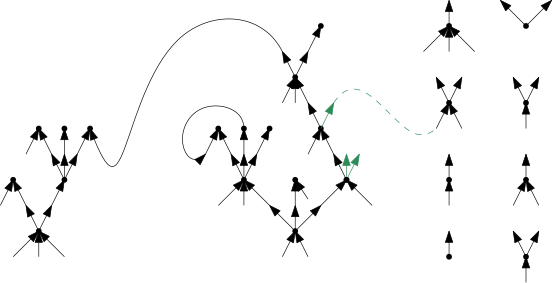
\includegraphics[scale=0.6]{Content/Pictures/Configuration model.png}
    \caption{The red arrows represent unpaired out-edges. One by one, in depth first order, these are connected to a uniform available in-edge.}
    \label{fig.configuration model}
\end{figure}
\begin{figure}
    \centering
    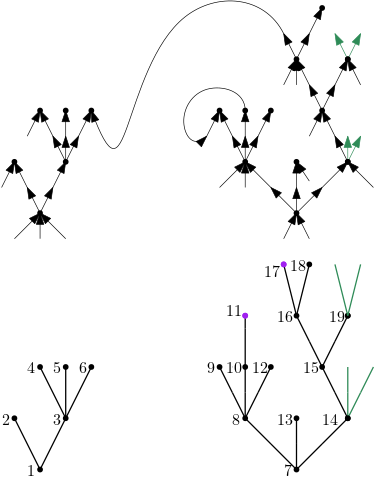
\includegraphics[scale=0.8]{Content/Pictures/Configuration model out-forest.png}
    \caption{By removing the surplus edges and in-edges we obtain the out-forest. For every sampled surplus edge, we add an extra leaf, which we colour purple. The red edges lead to vertices of which we do not know whether they are purple, and we do not know their degree yet. This corresponds to out-half-edges that have not been paired yet. The dashed lines are not part of the out-forest, but are there to illustrate the connection between the digraph and the out-forest.}
    \label{fig.configuration modeloutforest}
\end{figure}
\begin{enumerate}
    \item \label{cond.mu}$\E[D^+]=\E[D^-]=\mu$
    \item \label{cond.beta}$\E\left[(D^-)^2\right]=\beta<\infty$
     \item \label{cond.gamma}$\E\left[(D^-)^3\right]=\gamma<\infty$   \item \label{cond.critical} $\E[D^+ D^-]=\mu$
    \item \label{cond.rho} $\E\left[(D^+)^2 D^-\right]=\rho<\infty$
      \item \label{cond.tau} $\E\left[D^+ (D^-)^2\right]=\tau<\infty$
      \item \label{cond.iota} $\E\left[D^+(D^-)^3\right]=\iota<\infty$
\end{enumerate}
\begin{remark}
As noted earlier, in order for a digraph with a given degree sequence to exist, we need that the total number of in-edges is equal to the total number of out-edges. We hope that if the degree distribution satisfies condition \ref{cond.mu}, conditioning on an equal number of in-edges and out-edges does not effect the early stages of the exploration. 
Conditions \ref{cond.beta} and \ref{cond.gamma} ensure that the Central Limit Theorem applies to the fluctuations of the first explored in-degrees around their mean. Condition \ref{cond.critical} ensures that the branching process corresponding to the depth-first exploration (i.e. the exploration of the out-components) is critical. Condition \ref{cond.rho} ensures that this branching process has Brownian scaling. Condition \ref{cond.tau} ensures that the covariance of the in- and out-degrees that are discovered first is finite. Condition \ref{cond.iota} ensures that the strongly connected components are $3$-regular. 
\end{remark}
\subsection{Proof outline}


\subsection{Some first results}
\subsubsection{The in-degrees in order of discovery}
In our depth-first exploration, the next vertex is chosen with probability proportional to its in-degree. Hence, the sequence of in-degrees in order of discovery is a \emph{size-biased ordered sequence}. Denote the sequence of the first $m$ discovered vertices in order of discovery
$$(\hat{D}^-_1,\dots, \hat{D}^-_m).$$ Note that $\hat{D}_1^-,\dots , \hat{D}_m^-$ are not identically distributed or independent. This sequence is however closely related to a sequence of i.i.d.\ random variables with the size-biased distribution of $D^-$. Such a random variable $Z$ is distributed as $$\P(Z=k)=\frac{k\P(D^-=k)}{\E[D^-]}.$$
Proposition 4.2 in \cite{Conchon2018} identifies the measure change between $$(\hat{D}^-_1,\dots, \hat{D}^-_m)$$ and $$(Z_1^-,\dots,Z_m^-),$$ for $Z_1^-,\dots,Z_m^-$ i.i.d.\ random variables with the size-biased distribution of $D^-$. The content of the proposition is as follows.

\begin{proposition}\label{prop.measurechange}
For $m\leq n$ and $k_1,\dots,k_m\geq 1$, define
$$\phi_m^n(k_1,\dots,k_m)=\E\left[\prod\limits_{i=1}^m \frac{(n-i+1)\mu}{\sum_{j=i}^m k_j + \Xi_{n-m}}\right],$$
where $\Xi_{n-m}$ has the same law as $D^-_{m+1}+\cdots+D^-_n$. Then, for any suitable test function $g:\Z_+^m\to \R_+$, 
$$\E[g(\hat{D}^-_1,\dots, \hat{D}^-_m)]=\E[\phi_m^n(Z_1^-,\dots,Z_m^-)g(Z_1^-,\dots,Z_m^-)].$$
\end{proposition}

We fix $t>0$ and choose $m=\lfloor n^{2/3}t\rfloor$, and are interested in how the measure change in Proposition \ref{prop.measurechange} behaves if $n\to \infty$. This is the content of the next proposition. 
\begin{proposition}\label{prop.scalingmeasurechange}
Let $\Phi(n,m):=\phi_n^m(Z^-_1,\dots,Z^-_m)$. Then, for $\sigma=\left(\frac{\gamma-\beta^2/\mu}{\mu}\right)^{1/2}$, and $(B_s,s\geq 0)$ a standard Brownian motion, define $$\Phi(t)=\exp\left(-\frac{\sigma}{\mu}\int_0^tsdB_s - \frac{t^3 \sigma^2}{6\mu^2}\right).$$
Then, for fixed $t$, $\Phi(n,\lfloor  n^{2/3} t \rfloor)\overset{d}{\to}\Phi(t)$ as $n\to \infty$. Moreover, the sequence $(\Phi(n,\lfloor  n^{2/3} t \rfloor))_{n\geq1}$ of random variables is uniformly integrable. 
\end{proposition}
The proof of this statement is analogous to the proof of Lemma 6.7 in \cite{Conchon2018}.\\

Note that every time we discover a vertex with in-degree $d^-$ that is not the root of an out-component, we use one of its in-edges to connect to an out-edge of the last explored vertex. Hence, the \emph{stack} of seen, but unused in-edges increases by $d^--1$. If we ignore the times that an out-edge is matched to one of the in-edges on the stack, and ignore one of the in-edges of the root of every out-component, the process 
$$\hat{S}^-(k):=\sum\limits_{i=1}^k(\hat{D}^-_i-1)$$ keeps track of the stack size. We will investigate this process using the measure change from Proposition \ref{prop.measurechange}, so we define 
$${S}^-(k):=\sum\limits_{i=1}^k(Z^-_i-1).$$
However, note that $\E[Z^-_1]=\frac{\beta}{\mu}>1$, so ${S}^-(k)$ is an uncentred random walk. Hence,
\begin{equation}\label{eq.convergenceinprocess} (n^{-2/3}{S}^-(\lfloor n^{2/3}t\rfloor),t\geq 0) \overset{\P}{\to} \left(\frac{\beta-\mu}{\mu}t, t\geq 0\right)\end{equation}
in the Skorokhod topology as $n\to \infty$.
Combining this with Proposition \ref{prop.scalingmeasurechange} gives us that for every $T\geq 0$,
\begin{equation}\label{eq.convergenceorderedinedges} (n^{-2/3}\hat{S}^-(\lfloor n^{2/3}t\rfloor),0\leq t \leq T) \overset{\P}{\to} \left(\frac{\beta-\mu}{\mu}t, 0\leq t \leq T \right)\end{equation}
in the Skorokhod topology as $n\to \infty$.
Informally, the measure change only has an effect on the cumulative fluctuations of $Z_1,\dots,Z_m$ around their mean, which occur on a scale $n^{1/3}$. This is not observed on the scale of $\hat{S}^-(\lfloor n^{2/3}t\rfloor)$. However, if we examine the random fluctuations around the mean, we observe the following. 
\begin{equation}\label{eq.convergencein-edges}\left(n^{-1/3}{S}^-(\lfloor n^{2/3}t\rfloor)-\frac{\beta-\mu}{\mu}t ,t\geq 0\right) \overset{d}{\to} \left(\sigma B_t, t\geq 0\right).\end{equation}


Analogously to the proof of Theorem 4.1 in \cite{Conchon2018}, we can then show that for any $T\geq 0$,
$$\left(n^{-1/3}{\hat{S}}^-(\lfloor n^{2/3}t\rfloor)-\frac{\beta-\mu}{\mu}t ,0\leq t\leq T\right) \overset{d}{\to} \left( \hat{B}^-_t, 0\leq t \leq T \right),$$
where $(\hat{B}^-_t,0\leq t \leq T)$ is defined as follows. For $F$ a suitable test function, and for $(B_t)_{t\geq 0}$ a Brownian motion,
\begin{equation}\label{eq.measurechangeapplied} \E\left[F(\sigma\hat{B}^-_t,0\leq t \leq T)\right]=\E\left[\exp\left(-\frac{\sigma}{\mu}\int_0^T sdB_s - \frac{T^3 \sigma^2}{6\mu^2}\right)F(\sigma{B}_t,0\leq t \leq T)\right].\end{equation}
\subsubsection{The out-degrees in order of discovery}\label{subsubsection.out-degrees}
Fix $t$ and $n$ and set $m=\lfloor  n^{2/3} t\rfloor$. Suppose we sampled our sequence of in-degrees $(D^-_1,\dots,D_n^-)$. Then, we determined what the first $m$ in-degrees in our exploration are, namely $(\hat{D}_1^-,\dots,\hat{D}_m^-)$. The next step is to sample the corresponding out-degrees. Let $D^+_i(d^-)$ have the law of the out-degree of a vertex with in-degree $d^-$. If it were not possible for out-edges to connect to in-edges of vertices that were visited earlier in the exploration, the \L ukasiewicz process of depth-first exploration the out-components would be given by 
 $$ \hat{S}^+(k)=\sum\limits_{i=1}^k (D^+_i(\hat{D}^-_i)-1).$$
 We will again investigate this process via the measure change given in Proposition \ref{prop.measurechange}, so we define $$ {S}^+(k)=\sum\limits_{i=1}^k (D^+_i(Z^-_i)-1).$$ 
 Firstly, we see that by conditions \ref{cond.critical} and \ref{cond.rho} on the degree distribution, for $\lambda=\left(\frac{\rho-\mu}{\mu}\right)^{1/2}$ and $(B_t)_{t\geq0}$ a Brownian motion, \begin{equation} \label{eq.limitoutdegreecritical}\left(n^{-1/3}S^+(\lfloor n^{2/3}t\rfloor) ,t\geq 0\right)\overset{d}{\to}(\lambda B_t,t\geq 0).\end{equation}
 Since $S^-(k)$ converges to a deterministic function under scaling, the convergence in \eqref{eq.limitoutdegreecritical} holds jointly with the convergence in \eqref{eq.convergenceinprocess}. To understand how  the change of measure affects the out-process, we also need to study the joint distribution of  $\sum_{i=1}^m(Z^-_i-\beta/\mu)$ and $\sum_{i=1}^m(D^+_i(Z^-_i)-1)$ and their limits under scaling. This is the content of the following proposition.
\begin{proposition}
\label{prop.jointconvergenceinout}
 Like before, let $\sigma=\left(\frac{\gamma-\beta^2/\mu}{\mu}\right)^{1/2}$, and $\lambda=\left(\frac{\rho-\mu}{\mu}\right)^{1/2}$. Also define $\kappa=\frac{\tau-\beta}{\mu}$. Then,
 \begin{align*} &\left(n^{-1/3}\sum\limits_{i=1}^{\lfloor  n^{2/3}t\rfloor} \left(Z^-_i-\frac{\beta}{\mu}\right),n^{-1/3}\sum\limits_{i=1}^{\lfloor  n^{2/3} t\rfloor} \left(D^+_i(Z^-_i)-1\right), t\geq 0\right)\\
 &\overset{d}{\to} \left(\frac{\kappa}{\lambda}B_t^1+\left(\sigma^2-\frac{\kappa^2}{\lambda^2}\right)^{1/2}B_t^2   ,\lambda B_t^1, t\geq 0 \right)\end{align*}
 in the Skorokhod topology, as $n\to \infty$, with $(B^1_t)_{t\geq 0}$ and $(B^2_t)_{t\geq 0}$ two independent standard Brownian motions. 
\end{proposition} 
\begin{proof}
 Firstly, we notice that 
 \begin{align*}
     \E\left[\left(Z^-_1-\frac{\beta}{\mu}\right)^2\right]&=\sigma^2,\\
      \E\left[\left(D^+_1(Z^-_1)-1\right)^2\right]&=\lambda^2,\text{ and}\\
     \E\left[\left(Z^-_1-\frac{\beta}{\mu}\right)\left(D^+_1(Z^-_1)-1\right)\right]&=\kappa.\\
 \end{align*}
 Then, by Theorem 7.1.4 in \cite{Ethier1986}, we get that 
 $$\left(n^{-1/3}\sum\limits_{i=1}^{\lfloor  n^{2/3}t\rfloor} \left(Z^-_i-\frac{\beta}{\mu}\right),n^{-1/3}\sum\limits_{i=1}^{\lfloor  n^{2/3}t\rfloor} \left(D^+_i(Z^-_i)-1\right), t\geq 0\right)$$
 converges to a Gaussian process with covariance matrix
 $$A_t=\begin{pmatrix} \sigma^2  & \kappa \\ \kappa  & \lambda^2  \end{pmatrix}t,$$
 and we see that such a process is equal in law to
 $$\left(\frac{\kappa}{\lambda}B_t^1+\left(\sigma^2-\frac{\kappa^2}{\lambda^2}\right)^{1/2}B_t^2   ,\lambda B_t^1 ,t\geq 0\right).$$
 \end{proof}\\
 We are now able to examine the effect of the change of measure on the out-process. This is the content of the following theorem. 
\begin{theorem}\label{theorem.convaftermeasurechange} 
 For $\left(\hat{S}^-(k)\right)_{k\geq 0}$ encoding the in-degrees in order of discovery and   $\left(\hat{S}^+(k)\right)_{k\geq 0}$ encoding the out-degrees in order of discovery for the model on $n$ vertices, for $T>0$,
$$\left(n^{-2/3}\hat{S}^-\left(\lfloor n^{2/3} t\rfloor\right), n^{-1/3}\hat{S}^+\left(\lfloor  n^{2/3} t\rfloor\right), 0\leq t \leq T \right) \overset{d}{\to} \left( \frac{\beta-\mu}{\mu}t, \lambda\hat{B}_t^+, 0 \leq t \leq T \right)$$
in the Skorokhod topology as $n\to \infty$, where $(\hat{B}^+_t, t\geq 0)$ is distributed as follows.
For $F$ a suitable test function, and for $(B_t)_{t\geq 0}$ a Brownian motion,
\begin{align*} &\E\left[F(\lambda \hat{B}^+_t,0\leq t \leq T)\right]\\&=\E\left[\exp\left(-\frac{\kappa}{\lambda \mu} \int_0^T s dB_s -\frac{\kappa^2 T^3}{6\lambda^2 \mu^2}\right)F(\lambda B_t,   0\leq t \leq T)\right].\end{align*}

\end{theorem}
\begin{proof}
 Firstly, we use the results of Propositions \ref{prop.scalingmeasurechange} and \ref{prop.jointconvergenceinout}, and repeat the proof of Theorem 4.1 in \cite{Conchon2018} to find that for ${S}^{[n,-]}(t):=n^{-1/3}\sum_{i=1}^{\lfloor n^{2/3}t\rfloor} \left(\hat{D}^-_i-\frac{\beta}{\mu}\right) $ and ${S}^{[n,+]}(t):=n^{-1/3}\sum_{i=1}^{\lfloor  n^{2/3}t \rfloor} \left(\hat{D}^+_i(\hat{D}^-_i)-1\right)$, for $F$ a bounded continuous test-function,
 \begin{align*}&\E\left[F({S}^{[n,-]}(t),{S}^{[n,+]}(t), 0\leq t \leq T ) \right] \to \E\left[\Phi(T) F\left(\frac{\kappa}{\lambda}B_t^1+\left(\sigma^2-\frac{\kappa^2}{\lambda^2}\right)^{1/2}B_t^2   ,\lambda B_t^1, 0\leq t \leq T\right)\right]\\
 &= \E\left[\exp\left(-\frac{1}{\mu}\int_0^Tsd\left(\frac{\kappa}{\lambda}B_s^1+\left(\sigma^2-\frac{\kappa^2}{\lambda^2}\right)^{1/2}B_s^2\right) - \frac{T^3 \sigma^2}{6\mu^2}\right) F\left(\frac{\kappa}{\lambda}B_t^1+\left(\sigma^2-\frac{\kappa^2}{\lambda^2}\right)^{1/2}B_t^2   ,\lambda B_t^1, 0\leq t \leq T\right)\right]\end{align*}
 
 as $n\to \infty$. Hence, for $F$ a suitable test function, 
 \begin{align*}&\E\left[F({S}^{[n,+]}(t), 0\leq t \leq T ) \right]\\&\to \E\left[\exp\left(-\frac{\kappa}{\lambda \mu} \int_0^T s dB^1_s -\frac{\kappa^2 T^3}{6\lambda^2 \mu^2}\right)F(\lambda B^1_t,   0\leq t \leq T)\right].\end{align*}
 Combining this with \eqref{eq.convergenceorderedinedges} yields the result.
 \end{proof}\\
 The following lemma characterises the distribution of $(\hat{B}^+_t, {0\leq t\leq T})$.
 \begin{lemma}\label{lemma.characterizelimitprocess}
 For $(\hat{B}^+_t, {0\leq t\leq T})$ as in the statement of Theorem \ref{theorem.convaftermeasurechange}, we have that 
 $$(\lambda \hat{B}^+_t, {0\leq t\leq T})\overset{d}{=}\left(\lambda B_t-\frac{\kappa}{2\mu}t^2, {0\leq t\leq T}\right)$$
 for $(B_t)_{t\geq 0}$ a Brownian motion.
 \end{lemma}
 \begin{proof}
 Firstly, we see that for any $t\in [0,T]$ and $\theta>0$,
 \begin{align*} \E\left[\exp(-\theta \lambda \hat{B}_t^+)\right] &= \E \left[ \exp\left(-\frac{\kappa}{\lambda \mu}\int_0^t s dB_s-\frac{\kappa^2 t^3}{6\lambda^2\mu^2}-\theta\lambda B_t  \right)\right]\\
 &=\E\left[\exp \left( -\frac{\kappa}{\lambda \mu}\int_0^t \left(s+\frac{\lambda^2\theta \mu}{\kappa}\right) dB_s -\frac{\kappa^2 t^3}{6\lambda^2\mu^2}\right)\right] \\
 &= \exp\left(-\frac{\kappa^2}{2\lambda^2 \mu^2}\int_0^t \left(s+\frac{\lambda^2\theta \mu}{\kappa}\right)^2 ds -\frac{\kappa^2 t^3}{6\lambda^2\mu^2}\right)\\
 &=\exp\left(\frac{\lambda^2 t}{2}\theta^2+\frac{\kappa t^2}{2\mu}\theta \right)\\
 &= \E \left[\exp\left(-\theta\left(\lambda B_t - \frac{\kappa}{2\mu} t^2\right)\right)\right]
 \end{align*}
 for $(B_t)_{t\geq 0}$ a Brownian motion.
 Then, more generally, for $m>0$, $0=t_0\leq t_1\leq \cdots \leq t_m=T$, and $\theta_1, \dots, \theta_m \in \R_+$, 
 \begin{align*}
     &\E\left[\exp\left(-\sum_{i=1}^m \theta_i(\lambda\hat{B}_{t_i}^+-\lambda\hat{B}_{t_{i-1}}^+)\right)\right]\\
    %  &=\E \left[ \exp\left(-\frac{\sigma}{\mu} \sum_{i=1}^m \int _{t_{i-1}}^{t_i} s dB_s^1-\frac{\sigma^2}{2\mu^2}\sum_{i=1}^m \int_{t_{i-1}}^{t_i}s^2ds-\frac{ \kappa}{\sigma} \sum_{i=1}^m \theta_i(B_{t_i}^1-B_{t_{i-1}}^1)- 
    %  \left(\lambda^2-\frac{\kappa^2}{\sigma^2}\right)^{1/2}\sum_{i=1}^m \theta_i(B_{t_i}^2-B_{t_{i-1}}^2)\right)\right]\\
     &= \prod_{i=1}^m \E\left[\exp\left(-\frac{\kappa}{\lambda\mu} \int _{t_{i-1}}^{t_i} s dB_s-\frac{\kappa^2 (t_i^3-t_{i-1}^3)}{6\lambda^2 \mu^2}-\theta_i \lambda  (B_{t_i}-B_{t_{i-1}})\right)\right]\\
     &= \prod_{i=1}^m  \exp\left( -\frac{\kappa^2}{2\lambda^2 \mu^2}\int_{t_{i-1}}^{t_i}\left(s+\frac{\lambda^2\theta_i\mu}{\kappa}\right)^2 ds - \frac{\kappa^2 (t_i^3-t_{i-1}^3)}{6\lambda^2 \mu^2} \right)\\
     &=  \prod_{i=1}^m \exp\left(\frac{ \lambda^2 (t_i-t_{i-1}) }{2}\theta_i^2+\frac{\kappa (t_i^2-t_{i-1}^2)}{2\mu}\theta_i \right)\\
     &=\E \left[\exp\left(-\sum_{i=1}^m\theta_i\left(\lambda (B_t-B_{t_i}) - \frac{\kappa}{2\mu} (t_i^2-t_{i-1}^2)\right)\right)\right],
 \end{align*}
 which proves the result.
 
\end{proof}
 \subsection{Including surplus edges}
So far, we have not considered the possibility of out-edges connecting to in-edges of vertices that were visited earlier in the exploration. If that happens, we call such a pair of an in-edge and an out-edge a \emph{surplus edge}. An important fact, which we will prove later, is that at the moment a surplus edge is explored, we already know whether it will be part of a strongly connected component. This allows us to distinguish between two scenarios when a surplus edge from the $i^{th}$ out-edge of vertex $v$ to vertex $w$ is sampled.
\begin{enumerate}
    \item If the surplus edge is not part of a strongly connected component, we connect the $i^{th}$ out-edge of vertex $v$ to an extra leaf (see Figure \ref{fig.configuration modeloutforest}) and decrease the number of seen, but unmatched in-edges by $1$.
    \item If the surplus edge is part of a strongly connected component, we connect the $i^{th}$ out-edge of vertex $v$ to an extra leaf, decrease the number of seen, but unmatched in-edges by $1$, and take note that the extra leaf needs to be identified with vertex $w$. 
\end{enumerate}

We will now examine the different type of surplus edges we can encounter while exploring the out-forest. We distinguish between \emph{descendental surplus edges}, \emph{ancestral surplus edges} and \emph{additional surplus edges}. Descendental surplus edges point from a vertex $v$ to one of its descendants. Ancestral surplus edges point from a vertex $v$ to one of its ancestors. All other surplus edges are called additional surplus edges. This is illustrated in Figure \ref{subfigure.typesofsurplusedges}. In Figure \ref{subfigure.sccinexample} we show how surplus edges affect the structure of the strongly connected components. This is made rigourous in Lemma \ref{lemma.whatispartofscc}.
\begin{lemma}\label{lemma.whatispartofscc}
The following facts hold for strongly connected components. 
\begin{enumerate}
\item The vertices of a strongly component are contained in the vertices of one of the out-components.
\item Ancestral surplus edges are always part of a strongly connected component.
\item The event that a descendental or additional surplus edge is part of a strongly connected component is adapted to the history of the exploration up to the sampling of the surplus edge. 
\item For a descendental or additional surplus edge to be part of a strongly connected component, it is necessary that the starting point and endpoint of the edge are both contained in the same out-subtree rooted at the endpoint of an ancestral backedge.
\end{enumerate}
\end{lemma}
\begin{proof}
We start with the first statement. Let $v$ and $w$ be two vertices in the same strongly connected component. Without loss of generality, $v$ is explored first in depth-first order in the out-direction. By $v$ and $w$ being part of the same strongly connected component, we know that there is a path from $v$ to $w$ in the out-direction. This implies that $w$ will be part of the out-subtree rooted at $v$ and hence they are part of the same out-component. \\
To prove the second statement, suppose there is an ancestral surplus edge from $v$ to $w$. This implies that $w$ is an ancestor of $v$ in an out-component, which implies that there is a path from $w$ to $v$ as well. It follows that $w$ and $v$ are in the same strongly connected component and that the ancestral surplus edge from $v$ to $w$ is in this strongly connected component as well. \\
To prove the third statement, suppose that we sample a descendental surplus edge from $v$ to $w$. This implies that $w$ is a descendant of $v$ that we have already explored, and since our exploration is in depth-first order, we have also explored the out-subforest rooted at $w$. Any path from $w$ to one of the earlier vertices will be explored when the out-subtree rooted at $w$ is explored, so when the descendental surplus edge is sampled, we already know whether there is a path from $w$ to $v$. On the other hand, suppose we sample an additional surplus edge from $v$ to $w$. This implies that $w$ precedes $v$ in depth-first order in the out-direction, and since it is not an ancestor of $v$, the out-subtree rooted at $w$ is already fully explored and any path from $w$ to $v$ is already discovered. \\
For the last statement, note that any additional or descendental surplus edge from $v$ to $w$ is included in a strongly connected component if and only if there is path from $w$ to $v$ present at the time of sampling the surplus edge. Let $y$ be the smallest element in depth-first order on a path from $w$ to $v$, and let $x$ precede $y$ on this path, with $x\neq y$. This means that $y$ is less than or equal to $w$, $v$ and $x$ in depth first order, and since $w$, $v$ and $x$ can be reached from $y$, they must be contained in the out-subtree rooted at $y$. This also implies that $(x,y)$ is an ancestral backedge.
\end{proof}

\begin{figure}
\centering
\begin{subfigure}{0.7\textwidth}
 \centering
    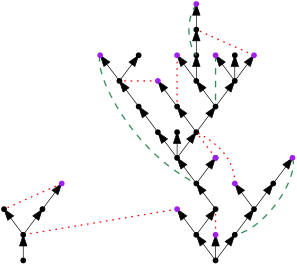
\includegraphics[width=0.7\linewidth]{Content/Pictures/Types of surplus edges.png}
    \label{subfigure.typesofsurplusedges} 
    \caption{This figure illustrates an example of a depth-first exploration of two out-components with the different type of surplus edges highlighted. The descendental surplus edges (blue) point from a vertex $v$ to one of its descendants. The ancestral surplus edges (green) point from a vertex $v$ to one of its ancentors. Any other surplus edge (red) is called an additional surplus edge.}
\end{subfigure}\\
\begin{subfigure}{0.7\textwidth}
  \centering
  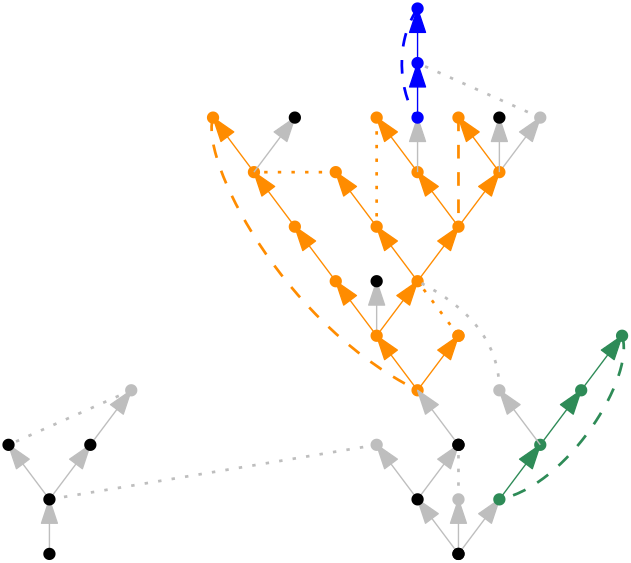
\includegraphics[width=0.7\linewidth]{Content/Pictures/SCC in example.png}
  \label{subfigure.sccinexample}
  \caption{The non-trivial strongly connected components embedded in the components of the out-forest are depicted in purple, darkgreen and orange. The trivial strongly connected components are black, and the grey edges are not part of a strongly connected component.}
\end{subfigure}
\caption{We illustrate the different types of surplus edges and how they affect the structure of the strongly connected components.}
\end{figure}




Note that a surplus edge can connect an out-edge to an in-edge in the same out-component, or to an in-edge in an earlier explored out-component. To incorporate surplus edges in our process, we need extra randomness. We will first modify the depth-first exploration encoded by $(S^+(k),S^-(k), k\leq m)$ to account for surplus edges. We will sample which out-edges are part of a surplus edge, and we will connect each of these to a special vertex with in-degree $1$ and out-degree $0$. We will sample which in-edges are part of a surplus edges by distorting distances in the tree, such that the new length measure represents the number of available in-edges in specific parts of the tree. We will then use the measure change to translate this to a modification of the depth-first exploration encoded by $(\hat{S}^+(k),\hat{S}^-(k), k\leq m)$. \\
However, in $(\hat{S}^+(k),\hat{S}^-(k), k\leq m)$, the sampling of surplus edges depends on the total number of in-edges available amongst all $n$ vertices, whereas we do not have such a stack available when we sample $(S^+(k),S^-(k), k\leq m)$. Therefore, we replace the total number of in-edges, i.e. $\sum_{i=0}^{n-1} D^-_i$, by $\mu n$, and later show that working with a deterministic 'stack size` does not affect the process on the scale that we are interested in. We denote the adaptation of $(S^+(k),S^-(k), k\leq m)$ in which surplus edges are accounted for, using the deterministic 'stack size`, by $(S^+_{eff}(k),S^-_{eff}(k), k\leq m)$. Denote the height process corresponding to $S^+_{eff}$ by $(H^+_{eff}(k), k\leq m)$. We will use an argument inspired by the method that Broutin, Duquesne and Wang employ in \cite{Broutin2020} to prove the following theorem. 
\myworries{In the below theorem, I will include the convergence of the height process encoding the metric structure on which the ancestral backedges are sampled on the length measure.}
\begin{theorem}\label{thm.convergenceSeff}
Let $(B_t,t\geq 0)$ be a Brownian motion and set $$(B^{eff}_t,t\geq 0)=\left(B_t-\frac{\beta - \mu}{2\lambda \mu^2}t^2,t\geq 0\right).$$ Then,
\begin{align*}
    &\left(n^{-1/3}S^+\left(\lfloor n^{2/3}t\rfloor\right),n^{-2/3}S^-\left(\lfloor n^{2/3}t\rfloor\right), n^{-1/3}S^+_{eff}\left(\lfloor n^{2/3}t\rfloor\right),\right.\\
    &\;\;\;\left.n^{-1/3}H^+_{eff}\left(\lfloor n^{2/3}t\rfloor\right), n^{-1/3}S^-_{eff}\left(\lfloor n^{2/3}t\rfloor\right), t\leq T\right)\\
    &\overset{d}{\to}\left(\lambda B_t, \frac{\beta-\mu}{\mu} t, \lambda B^{eff}_t,  \frac{2}{\lambda} \left(B^{eff}_{t}-\inf\{B^{eff}_{s}:s\leq t\}\right), \frac{\beta-\mu}{\mu} t, t\leq T\right)
\end{align*}
in $D([0,T],\R)^5$ as $n\to \infty$ . 
\end{theorem}

We investigate $(S^+_{eff}(k),S^-_{eff}(k), k\leq m)$ as follows. Fix $n$. We sample a
decorated Galton-Watson forest with offspring distributed as $D^+(Z^-_1)$ in a depth-first manner. The vertices are assigned a colour out of blue, purple and red, and every blue vertex has an in-degree associated to it. The forest is sampled in the following way. 
\begin{itemize}
    \item Whenever we explore a vertex, we decide on its colour before sampling its offspring.
    \item The first vertex of every component is blue.
    \item When we explore a blue vertex, we sample its in-degree and out-degree independent of everything else, distributed as $(Z_1^--1,D^+(Z_1^-))$. If the vertex is the root of a component, we add $1$ to its in-degree. The out-degree will play the role of the offspring of the vertex. 
    \item When we explore the child of a blue vertex, we decide whether the child is blue or purple. The purple vertices will play the role of the special vertices that we use to mark surplus edges. Hence, for every child of a blue vertex, the ratio of the 'seen but unused in-edges' and 'total unused in-edges' at the time that the child is explored, will be used as the probability that the child is purple. Since we do not actually have a stack of unseen in-edges, we set the total number of in-edges equal to $\mu n$. 
    \item When we explore a red or purple vertex, we sample its out-degree independent of everything else, distributed as $D^+(Z_1^-)$. 
    \item The children of purple and red vertices are all red.
    \end{itemize}  
The construction is illustrated in Figure \ref{fig.blueredpurpletrees}.

\begin{figure}
\centering
\begin{subfigure}{.5\textwidth}
  \centering
    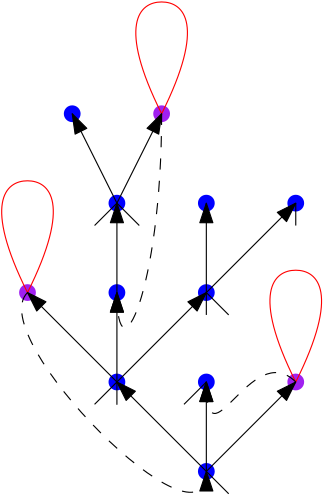
\includegraphics[width=.7\linewidth]{Content/Pictures/Blue-purple-red tree.png}
\end{subfigure}%
\begin{subfigure}{.5\textwidth}
  \centering
  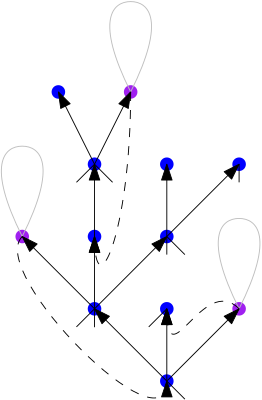
\includegraphics[width=.7\linewidth]{Content/Pictures/Blue purple tree.png}
\end{subfigure}
\caption{On the left hand side, we see how the Galton-Watson forest encoded by $X^+$ is constructed. A child of a blue vertex is purple with the probability of a surplus edge being found instead of the child. Therefore, for every purple vertex a dashed surplus edge is drawn. The pending red subtrees, encoded by excursions above the infimum of $X^{red,+}$, are represented by the red symbols. On the right hand side we illustrate how the blue purple forest is embedded in the Galton-Watson forest.}
\label{fig.blueredpurpletrees}
\end{figure}


We note that the blue-purple subforest is distributed as the out-forest encoded by $(S^+_{eff}(k),S^-_{eff}(k), k\leq m)$. Moreover, the \L ukasiewicz path and height process of the blue-purple subforest can be obtained from the \L ukasiewicz path and the height process of the blue-purple-red forest by skipping the intervals in which the red subtrees are explored. This is useful, because the convergence under scaling of the \L ukasiewicz path and height process of a Galton-Watson forest are well-understood, so if we show that the operation of skipping intervals behaves well under taking limits, we also obtain convergence under scaling of the \L ukasiewicz path and height process of the blue subforest. 
The precise definition of the process is as follows.
\begin{enumerate}
\item Sample $(X^{red,+}(k),k\geq 0)$ distributed as $(S^+(k),k\geq 0)$, which will encode the children of purple and red vertices. Independently, sample $(X^{blue,+}(k), X^{blue,-}_k,k\geq 0)$ distributed as $(S^+(k), S^-(k),k\geq 0)$, which will encode the in-degrees and out-degrees of the blue vertices. 
\item We will inductively define $(X^+(k), k\geq 0)$, which will be the \L ukasiewicz path of the Galton-Watson forest. We need to define a few time changes to sample offspring from either $X^{red,+}$ or $X^{blue,+}$ at the right times. Let $P(k)$ denote the number of purple vertices amongst the first $k$ explored blue and purple vertices, so we set $P(1)=0$. Define $\theta^{n}(k)=k-P(k-1)+\min\{j: X^{red,+}(j)=-P(k-1)\}$.  Note that $\min\{j: X^{red,+}(j)=-P(k-1)\}$ is the number of vertices in the first $P(k-1)$ components of the forest encoded by $X^{red,+}$, so if we identify their roots with the first $P(k-1)$ purple vertices, i.e. with the purple vertices amongst the first $k-1$ purple and blue vertices, then $\theta^{n}(k)$ is the total number of vertices explored until the exploration of the $k^{th}$ blue or purple vertex. Finally, we define $\Lambda^n(k)=\max\{j:\theta^{n}(j)\leq k\}-P(\max\{j:\theta^{n}(j)\leq k\})$. Note that $\max\{j:\theta^{n}(j)\leq k\}$ is the number of blue or purple vertices amongst the first $k$ vertices, so $\Lambda^n(k)$ is the number of blue vertices amongst the first $k$ vertices.
\item Define $I^+(k)=\min\{X^+(j) : j\leq k\}$.  Then, define 
$$p_{k+1}=\frac{X^{blue,-}(k-P(k))-I^+(\theta^{n}(k))-P(k)}{\mu n-k-I^+(\theta^{n}(k))}\one_{\left\{I^+(\theta^n(k-1))= I^+(\theta^n(k))\right\}},$$ which is the probability that $(k+1)^{th}$ blue or purple vertex to be explored is purple. Indeed, when the $(k+1)^{th}$ blue or purple vertex is about to be explored, $k-P(k)$ blue vertices have been explored, and their available in-edges are $X^{blue,-}(k-P(k))$ plus the number of roots explored so far, minus the $P(k)$ in-edges we have already used for surplus edges. The total number of in-edges still available are $\mu n$ minus the number of in-edges matched to a parent or as part of a surplus edge. The indicator ensures that the roots of the components are blue.
\item We now define \begin{equation}\label{eq.definitionX^+}X^+(k)=X^{blue,+}(\Lambda^n(k))+X^{red,+}(k-\Lambda^n(k)),\end{equation} and since the increments of $\Lambda^n$ have size $0$ or $1$, we see that the increments of $X^+$ are independent and are distributed as the increments of $S^+(k)$, so $X^+(k)$ is the \L ukasiewicz path of a Galton-Watson forest with offspring distributed as $D^+(Z^-_1)$. Let $(H(k),k\geq 0)$ be the height process corresponding to $X^+$. We also define $X^-(k)=X^{blue,-}(\Lambda^n(k))-P(\max\{j:\theta^{n}(j)\leq k\})-I^+(k)$, which is the number of seen, but unmatched in-edges after $k$ vertices have been explored. 
\item We see that $(H(\theta^{n}(k)),k\geq 0)$ corresponds to the height process of the blue and purple forest. $(X^+(\theta^{n}(k),k\geq 0)$ does however not exactly correspond to the \L ukasiewicz path of the blue and purple forest. Namely, if the $m^{th}$ blue or purple vertex is purple, $X^+(\theta^{n}(m)$ overcounts by the number of red children of this vertex. Hence, the \L ukasiewicz path of the blue and purple forest is encoded by \begin{equation}\label{eq.definitiontildeX}\tilde{X}^+(\theta^{n}(k)):=X^+(\theta^{n}(k))-E(\theta^{n}(k)),\end{equation}
where 
$E(\theta^{n}(k))$ counts the red children of the $\theta^n(k)^{th}$ vertex. We will argue that the size of $E$ is negligible on the scale we are interested in. $X^-(\theta^{n}(k))$ corresponds to the process encoding the available in-edges in the blue and purple forest.
\end{enumerate} 

 \begin{lemma}\label{lemma.tightnesssurplus edges}
 For every $T>0$, $$\left(n^{-1/3}P\left(\lfloor  n^{2/3}T\rfloor \right) \right)_{n\geq 1}$$ 
 is tight.
 \end{lemma}
 \begin{proof}
Set $m=\lfloor  n^{2/3}T\rfloor$ and fix $\epsilon>0$. For any $k\leq m$, the stack of unpaired seen in-edges after the first $k$ blue or purple vertices have been explored is bounded from above by $X^{blue,-}(k)+k$, which is the number of seen in-edges after the first $k$ blue vertices have been explored. The total number of unpaired in-edges after the first $k$ blue or purple vertices have been explored is bounded from below by $\mu n - k$, since any time a blue or purple vertex is explored, at most one in-edge is taken from the stack. Therefore, $$p_k\leq \frac{X^{blue,-}(k)+k}{\mu n - k},$$
and note that this upper bound is increasing in $k$. Consequently, conditional on $$(X^{blue,+}(j),X^{blue,-}(j),j\geq 0),$$ $n^{-1/3}P(m)$ is stochastically dominated by a binomial random variable with parameters  $X^{blue,+}(m)+m$ and $$\frac{X^{blue,-}(m)+m}{\mu n - m}\wedge 1.$$
Since $(X^{blue,+}(k)+k,k\geq 0)$ is a random walk with steps of finite mean, $\left(n^{-2/3}(X^{blue,+}(m)+m)\right)_{n\geq 1}$ is tight. Similarly, $\left(n^{-2/3}(X^{blue,-}(m)+m)\right)_{n\geq 1}$ is tight, and hence 
$$\left(n^{1/3} \frac{X^{blue,-}(m)+m}{\mu n - m}\right)_{n\geq 1}$$ is tight, which proves the statement.
\end{proof}\\
\begin{lemma}\label{lemma.convergenceQandP}
We have that 
$$\left(n^{-1/3}P(\lfloor n^{2/3}t\rfloor), t \geq 0\right)\overset{d}{\to} \left(\frac{\beta - \mu}{2\mu^2} t^2, t\geq 0\right)$$
in $D(\R_+,\R)$ as $n\to \infty$.

\end{lemma}
\begin{proof}
Fix $T>0$. We recall that $\theta^{n}(k):=k-P(k-1)+\min\{j: X^{red,+}(j)=-P(k-1)\}$. By tightness of $$\left(n^{-1/3}P\left(\lfloor  n^{2/3}T\rfloor \right) \right)_{n\geq 1},$$ by $(X^{red,+}(k), k\geq 0)$ being distributed as $(S^+(k),k\geq 0)$ and being downwards skip-free, and the convergence under scaling of $(S^+(k),k\geq 0)$ to a Brownian motion in \eqref{eq.limitoutdegreecritical}, also $\left(n^{-2/3}\theta^{n}(\lfloor n^{2/3}T\rfloor )\right)_{n\geq 1}$ is tight.  Since also $(X^+(k),k\geq 0)$ is distributed as $(S^+(k),k\geq 0)$, \eqref{eq.limitoutdegreecritical} and the continuous mapping theorem also yield tightness of $\left(n^{-1/3}I^+(\lfloor n^{2/3} t \rfloor)\right)_{n\geq 1}$ for all $t>0$, which implies that $\left(n^{-1/3}I^+(\theta^{n}(\lfloor n^{2/3} T \rfloor))\right)_{n\geq 1}$ is tight. \\
Recall that
$$p_{k+1}=\frac{X^{blue,-}(k-P(k))-I^+(\theta^{n}(k))-P(k)}{\mu n-k-I^+(\theta^{n}(k))}\one_{\left\{I^+(\theta^n(k-1))= I^+(\theta^n(k))\right\}}.$$
We will now argue that the indicator, which ensures that the roots are always blue, does not have an effect on $(P(k),k\leq m)$ on the scale we are interested in. Let $t>0$, and set $m=\lfloor n^{2/3}t\rfloor$. Define
\begin{align*}\begin{split}
E^p(m):&=\sum_{k=0}^{m-1} \frac{X^{blue,-}(k-P(k))-I^+(\theta^{n}(k))-P(k)}{\mu n-k-I^+(\theta^{n}(k))}\one_{\left\{I^+(\theta^n(k-1))\neq I^+(\theta^n(k))\right\}}\\
&\leq I^+(\theta^n(m)) \frac{X^{blue,-}(m)+m}{\mu n-X^{blue,+}(m)-m},\end{split}\end{align*}
so since $I^+(\theta^n(m))$ is of order $n^{1/3}$ and $\frac{X^{blue,-}(m)+m}{\mu n-X^{blue,+}(m)-m}$ of order $n^{-1/3}$, $(E^p(m))_{n\geq 1}$ is tight for all $t\geq 0$.  This means that without demanding that the roots are blue, we would only sample $O(1)$ purple roots up to time $O(n^{2/3})$, which does not effect $(P(k),k\leq m)$ on the scale we are interested in. \\
 Since $(X^{blue,-}(k),k\geq 0)$ is distributed as $(S^-(k),k\geq 0)$, the convergence in \eqref{eq.convergencein-edges} combined with the tightness of $(E^p(m))_{n\geq 1}$ implies that
\begin{equation}\label{eq.convergenceprob}\left(n^{1/3}p_{\lfloor n^{2/3} t \rfloor},t\geq 0\right)\overset{d}{\to} \left(\frac{\beta-\mu}{\mu^2}t,t\geq 0\right)\end{equation}
in $D(\R_+,\R)$ as $n\to \infty$. 
Then, by the continuous mapping theorem,
$$\left(n^{-1/3}\sum_{i=0}^{\lfloor n^{2/3}t \rfloor} p_k , t \geq 0\right)\overset{d}{\to} \left(\frac{\beta-\mu}{2\mu^2}t^2,t\geq 0\right)$$
in $D(\R_+,\R)$ as $n\to \infty$. \\
Let $\cF=(\cF_k,k\geq 0)$ denote the filtration such that $\cF_{k}$ contains the information on the shape of the forest until the exploration of the $k^{th}$ blue or purple vertex, including the colours of the vertices. To be precise,
$$\cF_k=\sigma\left((X^{blue,+}(l),X^{blue,-}(l), l\leq k-P(k),(X^{red,+}(l),l\leq \min\{m:X^{red,+}(m)=-P(k-1)\}), (P(l),l\leq k)\right).$$ Then, 
$$M(k):=\sum_{i=1}^k (\one_{\{P(i)-P(i-1)=1\}}-p_i)$$ is a martingale in $\cF$. We claim that $(n^{-1/3}M(\lfloor n^{2/3} t\rfloor ), t\geq 0)$ converges to $(0,t\geq 0)$ in probability in $D(\R_+,\R)$. Indeed, for any $t\geq 0$,
\begin{align*}\E[n^{-2/3}M(\lfloor n^{2/3} t\rfloor )^2]&=n^{-2/3}\sum_{i=1}^{\lfloor n^{2/3} t\rfloor} \E[\E[(\one_{\{P(i)-P(i-1)=1\}}-p_i)^2|\cF_{i-1}]]\\&=n^{-2/3}\sum_{i=1}^{\lfloor n^{2/3} t\rfloor} \E[p_i-p_i^2]\to 0.\end{align*}
Hence,
$$\left(n^{-1/3}P(\lfloor n^{2/3}t\rfloor), t\geq 0\right)=\left(n^{-1/3}\sum_{i=1}^{\lfloor n^{2/3}t\rfloor}  \one_{\{P(i)-P(i-1)=1\}}  , t\geq 0\right)\overset{d}{\to} \left(\frac{\beta - \mu}{2\mu^2} t^2, t\geq 0 \right),$$
 which proves the statement.

\end{proof}\\

\begin{lemma}\label{lemma.convergenceX+}
Let $(B^{blue}_t, t \geq 0)$ and $(B^{red}_t, t\geq 0)$ be two independent Brownian motions and let $$\theta(t):=t+\inf\left\{s\geq 0 : \lambda B^{red}_s< -\frac{\beta - \mu}{2\mu^2} t^2\right\},$$ and $\Lambda(t)=\inf\{s\geq 0:\theta(s)> t\}$. Define \begin{equation}\label{eq.definitionB^+}\left(B^+_t,t \geq 0\right):=\left( B^{blue}_{\Lambda(t)}+ B^{red}_{t-\Lambda(t)}, t\geq 0\right).\end{equation}
Then, $(G_t, t\geq 0):=\left(\frac{2}{\lambda}(B^+_t-\inf\{B^+_s,s\leq t\}),t\geq 0\right)$ is the height process corresponding to $\left(\lambda B^+_t,t \geq 0\right)$.
Moreover,
\begin{align}\begin{split}\label{eq.allencodingRVsconverge}&\left(n^{-1/3}X^{blue,+}\left(\lfloor n^{2/3}t \rfloor \right), n^{-1/3}X^{red,+}\left(\lfloor n^{2/3}t \rfloor \right),n^{-2/3} \Lambda^n\left(\lfloor n^{2/3}t\rfloor \right), \right.\\&\left.\,\,\,\,  n^{-1/3}X^+\left( \lfloor n^{2/3}t \rfloor \right), n^{-1/3}H\left( \lfloor n^{2/3}t \rfloor \right), n^{-2/3}\theta^n\left(\lfloor n^{2/3}t\rfloor \right),t\geq 0\right)\\
&\overset{d}{\to} \left(\lambda B^{blue}_t,\lambda B^{red}_t, \Lambda(t), \lambda B^+_{t} ,G_{t}, \theta(t), t\geq 0 \right)\end{split}\end{align}
in $D(\R_+,\R)^6 $ as $n\to \infty$. In particular,
\begin{equation}\label{eq.convergencecompX^+andtheta}\left(n^{-1/3}X^+\left(\theta^n \left(\lfloor n^{2/3}t\rfloor \right)\right), n^{-1/3}H\left(\theta^n\left(\lfloor n^{2/3}t\rfloor \right) \right),t\geq 0 \right) \overset{d}{\to} \left(\lambda B^+_{\theta(t)}, G_{\theta(t)},t\geq 0\right)\end{equation}
in $D(\R_+,\R)^2$ as $n\to \infty$ jointly with \eqref{eq.allencodingRVsconverge}.
\end{lemma}
\begin{proof} 
Firstly, note that by $X^+$ encoding a critical Galton-Watson forest with offspring variance $\lambda^2$, the proof of Theorem 1.8 in \cite{Legall2005} gives us that for $(B_s,s\geq 0)$ a Brownian motion,
\begin{equation}\label{eq.convergenceX}\left(n^{-1/3}X^+\left(\lfloor n^{2/3}s\rfloor \right), n^{-1/3}H\left(\lfloor n^{2/3}s\rfloor \right), s\geq 0 \right) \overset{d}{\to} \left(\lambda B_s,\frac{2}{\lambda} \left(B_s-\inf\{B_u:u\leq s\}\right),  s\geq 0\right) \end{equation}
 in $D(\R,\R)^2$ as $n\to \infty$, with $\left(\frac{2}{\lambda}(B^+_s-\inf\{B_u,u\leq s\}),s\geq 0\right)$ the height process corresponding to $\left(\lambda B_s,s \geq 0\right)$. Moreover, since $(X^{blue,+}(k),k\geq 0)\overset{d}{=}(X^{red,+}(k),k\geq 0)\overset{d}{=}(X^+(k),k\geq 0)$, and by \cite{Chaumont2010}, also
\begin{align}\begin{split}\label{eq.convergencebychaumont}&\left(n^{-1/3}X^{blue,+}\left(\lfloor n^{2/3} s \rfloor \right), n^{-1/3}X^{red,+}\left(\lfloor n^{2/3} s \rfloor \right), n^{-2/3}\inf\left\{k:n^{-1/3}X^{red,+}(k) \leq -x\right\}, s \geq 0, x\geq 0 \right)\\
&\overset{d}{\to}\left(\lambda B^{blue}(s), \lambda B^{red}(s), \inf\left\{u:\lambda B^{red}_u < -x\right\}, s\geq 0, x \geq 0\right)\end{split}\end{align}
in $D(\R_+,\R)^3$ as $n\to \infty$. Moreover, it is standard that 
\begin{equation}\label{eq.hittingtimestableprocess}\left(\inf\left\{u:\lambda B^{red}_u < -x\right\},x\geq 0\right)\overset{d}{=}\left(\frac{1}{\lambda^2}L_x,x\geq 0\right),\end{equation}
with $(L_x,x\geq 0)$ a stable subordinator with exponent $1/2$.
Since $P$ is non-decreasing, combining the convergence in \eqref{eq.convergencebychaumont} with Lemma \ref{lemma.convergenceQandP} gives that also
$$\left(n^{-2/3}\inf\left\{k:X^{red,+}(k) \leq - P\left(\lfloor n^{2/3} t \rfloor -1\right)\right\},t\geq 0\right)\overset{d}{\to}\left(\inf\left\{u:\lambda B^{red}_u< -\frac{\beta - \mu}{2\mu^2} t^2\right\},t\geq 0\right)$$
  in $D(\R_+,\R)$ as $n\to \infty$ jointly with the convergence in \eqref{eq.convergencebychaumont},
  and therefore, 
 \begin{equation}\label{eq.convergencetheta}\left(n^{-2/3}\theta^n\left(\lfloor n^{2/3}t\rfloor \right),t\geq 0 \right) \overset{d}{\to} \left(\theta(t),t\geq 0\right)\end{equation}
   in $D(\R_+,\R)$ as $n\to \infty$ jointly with the convergence in \eqref{eq.convergencebychaumont}.
Remember that 
$$\Lambda^n(k)=\max\{j:\theta^{n}(j)\leq k\}-P(\max\{j:\theta^{n}(j)\leq k\}). $$ By \eqref{eq.hittingtimestableprocess}, the jumps of $\left(\theta(t),t\leq T\right)$ are dense, and since $(\theta^n(k),k\geq 0)$ is increasing for all $n$ and $(\theta(t),t\geq 0)$ is increasing,  
$$\left(n^{-2/3}\max\{j:\theta^{n}(j)\leq \lfloor n^{2/3} t \rfloor\} ),t\geq 0\right)\overset{d}{\to}\left( \Lambda(t),t\geq0 \right)$$
in $D(\R_+,\R)$ as $n\to \infty$ jointly with the convergence in \eqref{eq.convergencebychaumont} and \eqref{eq.convergencetheta}. Since $\max\{j:\theta^{n}(j)\leq \lfloor n^{2/3} t \rfloor\}$ is of order $n^{2/3}$, Lemma \ref{lemma.tightnesssurplus edges} implies that also 
$$\left(n^{-2/3}\Lambda^n\left(\lfloor n^{2/3} t \rfloor\} \right),t\geq 0\right)\overset{d}{\to}\left( \Lambda(t),t\geq0 \right)$$
in $D(\R_+,\R)$ as $n\to \infty$ jointly with the convergence in \eqref{eq.convergencebychaumont} and \eqref{eq.convergencetheta}.\\
To finish the proof, we examine the construction of $(X^+(k),k\geq 0)$ in \eqref{eq.definitionX^+} and the construction of $(B^+_s,s\geq 0)$ in \eqref{eq.definitionB^+}. 
Note that $\Lambda^n(k)$ and $k-\Lambda^n(k)$ are non-decreasing. This implies that 
$$\left(n^{-1/3}X^+\left( \lfloor n^{2/3} t \rfloor \right), t\geq 0 \right)\overset{d}{\to} \left( B^+_{t}, t\geq 0\right)$$
in $D(\R_+,\R)$ as $n\to \infty$ jointly with all earlier mentioned converging random variables. Combining this with the joint convergence of $X^+$ with its height process shown in \eqref{eq.convergenceX} proves \eqref{eq.allencodingRVsconverge}. The fact that $(\theta^n(k),k\geq 0)$ is non-decreasing and composition of converging c\`adl\`ag functions then shows \eqref{eq.convergencecompX^+andtheta}.
\end{proof}
\begin{lemma}\label{lemma.subtracterrorconverges}
We have that 
$$\left(n^{-1/3}\tilde{X}^+\left(\theta\left(\lfloor n^{2/3}t\rfloor \right)\right), n^{-1/3}H\left(\theta\left(\lfloor n^{2/3}t\rfloor \right) \right),t\geq 0 \right) \overset{d}{\to} \left(\lambda B^+_{\theta (t)},\frac{2}{\lambda} \left(B^+_{\theta (t)}-\inf\{B^+_{s}:s\leq \theta(t)\}\right) ,t\geq 0 \right)$$
in $D(\R_+,\R)^2$ as $n\to \infty$. 


\end{lemma}
\begin{proof}
By the definition of $\tilde{X}^+$ in \eqref{eq.definitiontildeX}, and by Lemma \ref{lemma.convergenceX+}, it is sufficient to show that for any $T>0$,
$$n^{-1/3}\max_{k\leq \lfloor n^{2/3}T\rfloor}E(\theta^{n}(k))\overset{p}{\to}0.$$
We remind the reader that $E(k)$ counts the number of red children of $k^{th}$ visited vertex, so
$$n^{-1/3}\max_{k\leq \lfloor n^{2/3}T\rfloor}E(\theta^{n}(k))\leq n^{-1/3}\max_{k\leq \theta^{n}(\lfloor n^{2/3}T\rfloor)}(X^+(k)-X^+(k-1)+1),$$
which converges to $0$ by tightness of $\left(n^{-2/3}\theta^{n}(\lfloor n^{2/3}T\rfloor)\right)_{n\geq 1}$ and the fact that $$\left(n^{-1/3}X^+\left(\lfloor n^{2/3}t\rfloor\right),t\geq 0\right)$$ converges in distribution to a continuous process in $D(\R_+,\R)$ as $n\to\infty$.
\end{proof}

\begin{lemma}\label{lemma.heightprocesstimechange}
We have that with probability $1$, $$\left(\frac{2}{\lambda} \left(B^+_{\theta (t)}-\inf\{B^+_{s}:s\leq \theta(t)\}\right), t\leq T \right)=\left(\frac{2}{\lambda} \left(B^+_{\theta (t)}-\inf\{B^+_{\theta(s)}:s\leq t\}\right), t\leq T \right),$$ which is continuous, and it is the height process corresponding to $\left(\lambda B^+_{\theta (t)},t\leq T\right)$. 
\end{lemma}
\begin{proof}
From \cite{Legall2005}, we know that $(G(t),t\geq 0):=\left(\frac{2}{\lambda} \left(B^+_{t}-\inf\{B^+_{s}:s\leq t\}\right)  t\geq 0 \right)$ is the height process corresponding to $\left(\lambda B^+_{t},t\geq 0\right)$. By definition of the height process, we prove the statement if we show that with probability $1$, $(B^+_{\theta(t)},t\geq 0)$ is continuous, and for all $t\geq 0$, for all $s$ such that $\theta(t-)<s<\theta(t)$, $ B^+_s > B^+_{\theta(t)}$. \\
Recall that $(B^{blue}_t, t \geq 0)$ are $(B^{red}_t, t\geq 0)$ two independent Brownian motions and  $$\theta(t)=t+\inf\left\{s\geq 0 : \lambda B^{red}_s< -\frac{\beta - \mu}{2\mu^2} t^2\right\},$$ and $\Lambda(t)=\inf\{s\geq 0:\theta(s)> t\}$. Then, \begin{equation*}\left(B^+_t,t \geq 0\right):=\left( B^{blue}_{\Lambda(t)}+ B^{red}_{t-\Lambda(t)}, t\geq 0\right).\end{equation*}
Firstly, note that the jumps of $\theta$ correspond to excursions above the infimum of $B^{red}$.  With probability $1$, for all these excursions, the minimum on the excursion is only attained at the endpoints. This can be seen by uniqueness of local minima of Brownian motion, or by \^Ito excursion theory and the corresponding property for Brownian excursions. We will assume that this holds.\\
Now fix $t$ such that $\theta(t-)\neq \theta(t)$ and let $s\in (\theta(t-),\theta(t))$. Observe that $\Lambda$ is equal to $t$ on $[\theta(t-),\theta(t)]$. For $[\theta(t-),\theta(t))$ this follows by definition of $\Lambda$, and for $\theta(t)$ this follows by $\theta$ being strictly increasing. This implies that $$s-\Lambda(s)<\theta(t)-\Lambda(\theta(t))=\inf\{ u\geq 0: \lambda B_u^{red}<-(\beta-\mu)t^2/(2\mu^2)\}.$$ By our assumption on the minima on the excursions above the infimum of $B^{red}$, this implies that $$B^{red}_{s-\Lambda(s)}>-\frac{\beta - \mu}{2\mu^2} t^2=B^{red}_{\theta(t)-\Lambda(\theta(t))},$$
where the last equality follows from continuity of $B^{red}$. Combining this with $\Lambda(s)=\Lambda(\theta(t))$ implies that
$B^+_s>B^+_{\theta(t)}$. \\
Finally, 
$$B^+_{\theta(t-)}=B^{blue}_{\Lambda(\theta(t-))}+B^{red}_{\theta(t-)-\Lambda(\theta(t-))}
=B^{blue}_{t}+B^{red}_{\theta(t-)-t}$$
and by continuity of $B^{red}$,
\begin{align*}B^{red}_{\lim_{s\uparrow t}\inf\{u:B^{red}_u<-(\beta-\mu)s^2/(2\mu^2)\}}&=\lim_{s\uparrow t} B^{red}_{\inf\{u:B^{red}_u<-(\beta-\mu)s^2/(2\mu^2)\}}\\&= -\frac{\beta-\mu}{2\mu^2}t^2\\
&=B^{red}_{\theta(t)-t}, \end{align*}
so 
$B^+_{\theta(t-)}=B^+_{\theta(t)}.$
\end{proof}

We are now ready to prove Theorem \ref{thm.convergenceSeff}.

\begin{proofof}{\emph{Theorem \ref{thm.convergenceSeff}}}
The only missing ingredient is the law of $S^+_{eff}$ and $S^-_{eff}$. If we set $$(S^+(k),S^-,k\geq 0) =(X^{blue,+}(k),X^{blue,-}(k),k\geq 0),$$
then $S^+_{eff}$ corresponding to $S^+$ is distributed as the \L ukasiewicz path of the blue and purple forest corresponding to $X^{blue,+}$. Then, the process that keeps track of the unmatched in-edges of explored vertices is distributed as $S^-_{eff}$. 
Note that in this case 
$$S^+_{eff}(k)=X^{blue,+}(k-P(k))-P(k).$$
Indeed, at time $k$, the first $k-P(k)$ blue vertices have been explored, all contributing their degree minus $1$ to the sum, and $P(k)$ purple vertices have been explored, all contributing $-1$ to the sum. Using Lemma \ref{lemma.convergenceQandP}, we see that 
\begin{align*}
    \left(n^{-1/3}S^+\left(\lfloor n^{2/3}t\rfloor\right), n^{-1/3}S^+_{eff}\left(\lfloor n^{2/3}t\rfloor\right), t\geq 0\right)\overset{d}{\to}\left(\lambda B_t, \lambda B^{eff}_t, t\geq 0\right).
\end{align*}
in $D(\R_+,\R)^2$ as $n\to \infty$. 
By Lemma \ref{lemma.subtracterrorconverges} and Lemma \ref{lemma.heightprocesstimechange}, we know that $(S^+_{eff}(k),k\leq m)$ converges jointly with its height process, which implies that 
\begin{align*}
    &\left(n^{-1/3}S^+\left(\lfloor n^{2/3}t\rfloor\right), n^{-1/3}S^+_{eff}\left(\lfloor n^{2/3}t\rfloor\right),n^{-1/3}H^+_{eff}\left(\lfloor n^{2/3}t\rfloor\right), t\geq 0\right)\\
    &\overset{d}{\to}\left(\lambda B_t, \lambda B^{eff}_t,  \frac{2}{\lambda}\left(B^{eff}_{t}-\inf\{B^{eff}_{s}:s\leq t\}\right), t\geq 0\right).
\end{align*}
To conclude, we note that 
$$S^-_{eff}(k)=S^-(k-P(k))-P(k),$$
so \eqref{eq.convergenceinprocess} and Lemma \ref{lemma.convergenceQandP} imply the statement. 

\end{proofof}

We now want to use Theorem \ref{thm.convergenceSeff} to obtain convergence of $(\hat{S}^+(k),\hat{S}^-(k), k\leq m)$.  This is the content of the following theorem.
\begin{theorem}\label{thm.convergencetohatBeff}
Let $(B_t)_{t\geq 0}$ be a Brownian motion. Moreover, define
$$(\hat{B}^{eff}_t,t\geq 0):=\left( B_t-\frac{\tau-\mu}{2\lambda \mu^2}t^2, t\geq 0\right).$$ Then,

$$\left(n^{-1/3}\hat{S}^+_{eff}\left(\lfloor n^{2/3}t\rfloor \right),n^{-1/3}\hat{H}^+_{eff}\left(\lfloor n^{2/3}t\rfloor \right), t\geq 0\right)\overset{d}{\to}\left(\lambda \hat{B}^{eff}_t, \frac{2}{\lambda} \left(\hat{B}^{eff}_t-\inf\left\{\hat{B}^{eff}_s: s\leq t\right\}\right), t\geq 0\right)$$
as $n\to \infty$ in $\D(\R_+,\R)^2$ jointly with 
$$\left(n^{-2/3}\hat{S}^-_{eff}\left(\lfloor n^{2/3}t\rfloor \right), t\geq 0\right)\overset{p}{\to}\left(\frac{\beta-\mu}{\mu}t, t\geq 0\right)$$
as $n\to \infty$ in $\D(\R_+,\R)$.


\end{theorem}
\begin{remark}
Note that the coefficient of the parabolic drift is non-positive, i.e. $\tau\geq \mu$. Note that 
$$\frac{\E[D^+(D^-)^2]}{\E[D^+]}-\left(\frac{\E[D^+D^-]}{\E[D^+]}\right)^2=\frac{\tau}{\mu}-1$$
is the variance of $D^-$ under the law of the degree tuple size-biased by out-degree, which is non-negative. Hence $\tau/\mu\geq 1$, which shows that $(\hat{B}^{eff}_t)_{t\geq 0}$ is a Brownian motion with a downwards parabolic drift. 
\end{remark}
\begin{proof}
For all $k\geq 0$, let $B(k)$ denote the number of surplus edges in the first $k$ time-steps. This corresponds to $P(k)$ in our earlier construction. Define $C(k):=\inf\{l\leq k-B(k) :  \hat{S}^+(l)-B(l)\}$, and note like $I^+(\theta^n(k))$ in the definition of $p_{k+1}$, this corresponds to the number of roots after $k$ time steps.  Then, the actual probability forming a surplus edge in the $(k+1)^{th}$ time step is
$$q_k:=\frac{\hat{S}^-(k-B(k))-C(k)-B(k)}{\sum_{i=0}^n D^-_i-k-C(k)}\one_{\left\{C(k-1)= C(k)\right\}}.$$

Also define 

$$\tilde{q}_k:=\frac{\hat{S}^-(k-\tilde{B}(k))-\tilde{C}(k)-\tilde{B}(k)}{\mu n-k-\tilde{C}(k)}\one_{\left\{\tilde{C}(k-1)=\tilde{C}(k)\right\}},$$
where $\tilde{B}(k)$ is the number of surplus edges sampled if the probability of sampling a surplus edge instead of sampling the $(k+1)^{th}$ vertex is $\tilde{q}_k$ instead of ${q}_k$, and $\tilde{C}(k)$ is the number of roots in this process.
We claim that there exists a coupling such that
$$\sum_{i=0}^{\lfloor n^{2/3}T\rfloor }|q_i-\tilde{q}_i|\overset{p}{\to}0$$
as $n\to \infty$. 
Indeed, note that by earlier results and absolute continuity, 
$$\left(n^{-2/3}\max_{k\leq \lfloor n^{2/3}T\rfloor}(\hat{S}^-(k-B(k))-C(k)-B(k))\right)_{n>0}$$ is tight. Moreover by repeating the proof of Lemma \ref{lemma.tightnesssurplus edges}, we can show that $\left(n^{-1/3}\tilde{B}\left(\lfloor n^{2/3}T\rfloor \right)\right)_{n>0}$ is tight. This, combined with the convergence under scaling of $\hat{S}^+$, implies that also $\left(n^{-1/3}\tilde{C}\left(\lfloor n^{2/3}T\rfloor \right)\right)_{n>0}$ is tight.  By $D^+_1,\dots,D^+_n$ being i.i.d. random variables with mean $\mu$ and finite variance,
$\left(n^{-1/2}\left(\sum_{i=0}^{n-1}D^-_i-\mu n\right)\right)_{n>0}$ is tight. By using the trivial identity $a/b-c/d=(b(a-c)-c(d-b))/bd$, this implies that
$\left(n^{2/3}\max_{k\leq \lfloor n^{2/3}T\rfloor }|q_k-\tilde{q}_k|\right)_{n>0}$ is tight, which implies that there exists a coupling such that $\left(\max_{k\leq \lfloor n^{2/3}T\rfloor } |B(k)-\tilde{B}(k)|\right)_{n>1}$ and $\left(\max_{k\leq \lfloor n^{2/3}T\rfloor } |C(k)-\tilde{C}(k)|\right)_{n>1}$ are tight, which implies that, again by $a/b-c/d=(b(a-c)-c(d-b))/bd$, 
$\left(n^{5/6}\max_{k\leq \lfloor n^{2/3}T\rfloor }|q_k-\tilde{q}_k|\right)_{n>0}$ is tight, which implies that 
$$\sum_{i=0}^{\lfloor n^{2/3}T\rfloor }|q_i-\tilde{q}_i|\overset{p}{\to}0$$
as $n\to \infty$. 
Therefore, under the right coupling, 
$$\P\left(\max_{k\leq \lfloor n^{2/3} T \rfloor}|B(k)-\tilde{B}(k)|>0\right)\to 0.$$
In other words, we can couple the actual process that samples the graph to a process in which we replace the probability of sampling a surplus edge by $\tilde{q}_k$, in such a way that we do not see the difference on the scale that we are interested in. Therefore, we can replace $q_k$ by $\tilde{q}_k$. In that case, the sample paths of $(\hat{S}^+_{eff}(k),\hat{S}^-_{eff}(k), \hat{H}^+_{eff}(k), k \leq \lfloor n^{2/3}T\rfloor )$ are constructed out of sample paths of $(\hat{S}^+(k),\hat{S}^-(k), k\leq \lfloor n^{2/3}T\rfloor )$ and independent randomness in the exact same way as the sample paths of $({S}^+_{eff}(k),{S}^-_{eff}(k), {H}^+_{eff}(k), k \leq \lfloor n^{2/3}T\rfloor )$ are constructed out of sample paths of $({S}^+(k),{S}^-(k), k\leq \lfloor n^{2/3}T\rfloor )$ and independent randomness. 
We will use the following notation:\begin{align*}
    \hat{S}_{eff}^{(n)}&:=\left(n^{-1/3}\hat{S}^+_{eff}\left(\lfloor n^{2/3} t \right),0\leq t \leq T\right)\\
    \hat{H}_{eff}^{(n)}&:=\left(n^{-1/3}\hat{H}^+_{eff}\left(\lfloor n^{2/3} t \right),0\leq t \leq T\right)\\
    \hat{S}^{(n)}&:=\left(n^{-1/3}\hat{S}^+\left(\lfloor n^{2/3} t \right),0\leq t \leq T\right)\\
     {S}_{eff}^{(n)}&:=\left(n^{-1/3}{S}^+_{eff}\left(\lfloor n^{2/3} t \right),0\leq t \leq T\right)\\
    {H}_{eff}^{(n)}&:=\left(n^{-1/3}{H}^+_{eff}\left(\lfloor n^{2/3} t \right),0\leq t \leq T\right)\\
    {S}^{(n)}&:=\left(n^{-1/3}{S}^+\left(\lfloor n^{2/3} t \right),0\leq t \leq T\right).
\end{align*}
Let $f:D([0,T],\R)^2\to \R$ be a bounded, continuous test-function. Then,
\begin{align*}\E\left[f\left(\hat{S}_{eff}^{(n)},  \hat{H}_{eff}^{(n)}\right) \right]&= \E\left[ \E\left[\left. f\left(\hat{S}_{eff}^{(n)},  \hat{H}_{eff}^{(n)}\right)\right|\hat{S}^{(n)}\right]\right]\\&=\E\left[ \Phi(n,\lfloor n^{2/3} t\rfloor)\E\left[\left.f\left({S}_{eff}^{(n)},  {H}_{eff}^{(n)}\right)\right| {S}^{(n)}\right]\right]\\&=\E\left[ \Phi(n,\lfloor n^{2/3} t\rfloor)f\left({S}_{eff}^{(n)},  {H}_{eff}^{(n)}\right)\right],\end{align*}
where we use that $\E\left[\left. f\left(\hat{S}_{eff}^{(n)},  \hat{H}_{eff}^{(n)}\right)\right|\hat{S}^{(n)}\right]$ is a bounded, adapted function of $\hat{S}^{(n)}$, and that $\Phi(n,\lfloor n^{2/3} t\rfloor)$ is the measure change from ${S}^{(n)}$ to $\hat{S}^{(n)}$. Then, using Proposition \ref{prop.measurechange}, Proposition \ref{prop.scalingmeasurechange} and Theorem \ref{thm.convergenceSeff}, following the proof of Theorem 4.1 in \cite{Conchon2018} gives us that 
\begin{align*}
    &\E\left[f\left(\hat{S}_{eff}^{(n)},  \hat{H}_{eff}^{(n)}\right) \right]\\
    &\to \E\left[\Phi(t)f\left(\lambda B_t^{eff},\frac{2}{\lambda}\left(B_t^{eff}-\inf\left\{B_s^{eff}:s\leq t\right\}\right),0\leq t \leq T\right)\right].
\end{align*}
Since $$(B^{eff}_t,t\geq 0)=\left(B_t-\frac{\beta - \mu}{2\lambda \mu^2}t^2,t\geq 0\right),$$
Lemma \ref{lemma.characterizelimitprocess} implies the joint convergence of $\hat{S}^+_{eff}$ and $\hat{H}^+_{eff}$. By Theorem \ref{thm.convergenceSeff}, $S^-_{eff}$ converges in distribution to a deterministic process under scaling, which will not be effected by the measure change. This completes the proof. 
\end{proof}

Later on, we will want to extract excursions of $(\hat{S}_{eff}^+(k), k\geq 0)$, for which we need to consider $\hat{S}^+_{eff}$ reflected at its minimum, i.e.
$$(\hat{R}^n_{eff}(k),k\geq 0):=\left(\hat{S}_{eff}^+(k)-\min\left\{\hat{S}_{eff}^+(m):m\leq k\right\},k\geq 0\right).$$ We let $(\hat{C}^n_{eff}(k), k\geq 0)$ keep track of the number of excursions of $\hat{S}^+_{eff}$ above its infimum, i.e.
$$(\hat{C}^n_{eff}(k),k\geq 0):=\left(-\min\left\{\hat{S}_{eff}^+(m):m\leq k\right\},k\geq 0\right).$$
\begin{corollary}\label{cor.convergencereflected}
We have that for 
$$(\hat{R}^{eff}_t,t\geq 0):=\left(\lambda \hat{B}^{eff}_t-\lambda\inf\left\{\hat{B}^{eff}_s, s\leq t\right\},t\geq 0\right)$$
and
$$(\hat{C}^{eff}_t,t\geq 0):=\left(-\lambda\inf\left\{\hat{B}^{eff}_s, s\leq t\right\},t\geq 0\right),$$
that, jointly with the convergence in Theorem \ref{thm.convergencetohatBeff},
$$\left(n^{-1/3}\hat{R}^n_{eff}\left(\lfloor n^{2/3}t\rfloor\right),n^{-1/3}\hat{C}^n_{eff}\left(\lfloor n^{2/3}t\rfloor\right), t\geq 0\right)\overset{d}{\to}\left(\hat{R}^{eff}_t,\hat{C}^{eff}_t,t\geq 0\right)$$
in $D(\R_+,\R)$ as $n\to \infty$.
\end{corollary}
\begin{proof}
This follows from Theorem \ref{thm.convergencetohatBeff} and the continuous mapping theorem.
\end{proof}



% $$\P(\Xi_n>y)\sim \frac{e^{-vy}\P(\Xi_n\leq 1)}{1-e^{-v}}.$$

% Summing over strongly connected components yields
% $$\limsup_n\frac{q(n,[y,\infty))}{q(n,[0,1])}\leq \sup_{v\geq \delta}\frac{e^{-vy}}{1-e^{-v}}=\frac{e^{-\delta y}}{1-e^{-\delta}}.$$
% Because the size of a strongly connected component is smaller than its total in-degree, we see that $p(n,y,\delta)\leq q(n,[y,\infty))$, so it suffices to prove that 
% $$\sup_{n}q(n,[0,1])<\infty.$$
% We see that the number of strongly connected components with total in-degree at least $\delta n^{1/3}$ that are first discovered before time $n^{2/3}$ is bounded above by the sum of the number of vertices with in-degree at least $\delta n^{1/3}$ discovered before time $n^{2/3}$ and the number of ancestral backedges in the components of the out-forest that are visited before time $n^{2/3}$. To bound the first term in this sum, notice that for $(D^-,D^+)$ a random variable with the degree distribution, 
% $$\P(D^-\geq \delta n^{1/3})\leq \frac{\E[(D^-)^3]}{\delta^3 n}=\frac{\gamma}{\delta^3 n},$$
% which implies that 
% $$\E[\#\text{ vertices with in-degree }\geq \delta n^{1/3}]\leq \frac{\gamma}{\delta^3}<\infty.$$
% To bound the second term, note that conditional on the XXX
% \myworries{Prove this.}

\end{proof}
\subsection{Excursion theory}\label{subsec.excursiontheory}

% \myworries{Mimic section 3.2 of Christina's paper, include additivity result of paper with Robin}
We will use the following notation. The description will closely follow Subsection 3.2 in \cite{Conchon2018}. Write $D(\R_+,\R_+)$ for the space of c\`adl\`ag functions $f:\R_+\to \R_+$. We will write $\cE$ for the space of excursions, i.e.
$$\cE=\left\{\varepsilon \in D(\R_+,\R_+):\exists t>0\text{ s.t. }\varepsilon(s)>0\text{ for }s\in (0,t)\text{ and }\varepsilon(s)=0\text{ for }s\geq t\right\}.$$
For $\varepsilon\in \cE$, let $\zeta(\varepsilon)$ be the lifetime of $\varepsilon$, i.e. the smallest $t$ such that $\varepsilon(s)=0$ for $s\geq t$. Let $\cE^*=\cE\cup\{\delta\}$, where $\delta$ represents the empty excursion, with $\zeta(\delta)=0$. We will decompose $(\lambda \hat{B}^{eff}_t,t\geq 0)$ into excursions above the running infimum, since these excursions will encode the components of the limiting $\R$-forest. Set $I_t=\inf_{0\leq s\leq t}\lambda \hat{B}_t^{eff}$, which is a local time at zero for 
$$(R_t,t\geq 0)=\left(\lambda \hat{B}_t^{eff}-\inf_{0\leq s \leq t}\lambda \hat{B}_s^{eff},t\geq 0\right)$$  and write $\sigma _l=\inf\{t\geq 0: I_t<-l\}$, so that $(\sigma_l, l\geq 0)$ is the inverse local time. Then, write 
$$\varepsilon^{(l)}=\begin{cases}(R_{\sigma_{l-}+u}, 0\leq u \leq \sigma_l-\sigma_{l-})&\text{ if }\sigma_l-\sigma_{l-}>0\\ \delta &\text{otherwise.}\end{cases}.$$
\myworries{Results like in Subsection 3.2 in \cite{Conchon2018} follow from the fact that the limiting process is of the form $(c_1 B_t-c_2 t^2,t\geq 0)$ and results on excursions of spanning forest of $G(n,1/n)$}
% We will use the following facts about $(R_t,t\geq 0)$, that are proved in \cite{Conchon2018} as Lemma 3.5 in a more general setting, also covering a family of processes that are locally absolutely continuous to an $\alpha$-stable L\'evy process. 
% \myworries{Maybe find another reference/easy proof for these facts - should be pretty straightforward?}
% \begin{lemma}\label{lemma.propertiesexcursions}
% \begin{enumerate}
%     \item For each $\epsilon >0$, $R$ has only finitely many excursions of length greater than or equal to $\epsilon$.
%     \item The set $\{t:R_t=0\} $ has Lebesgue measure $0$.
%     \item If $(l_1,r_1)$ and $(l_2,r_2)$ are excursion intervals of $R$ and $l_1<l_2$, then $\hat{B}^{eff}_{l_1}>\hat{B}^{eff}_{l_2}$. 
% \end{enumerate}
% \end{lemma}
% The first part of this lemma allows us to list the excursions of $R$ in decreasing order of length. Write $(\varepsilon_i, i\geq 1)$ for this list. Write $(h_i,i\geq 1)$ for the corresponding height process excursions. 

% \myworries{Include equivalent of Proposition 3.8 and 3.9 of Christina's paper, using the measure change below. Note that excursions have same distribution as excursions in scaling limit of $G(n,p)$}



\subsection{Component-wise convergence}
This section is devoted to showing that the sequence of encoding excursions ordered by excursion length converges. Set $\sigma^n(0)=0$ and for $k\geq 1$, set
$$\sigma^n(k)=\inf\{j\geq 0: I^n(j)\leq -k\},$$
where $I^n(k)=\min_{j\leq k}\{\hat{S}^+_{eff}(j)\}$, so that $\sigma^n(k)$ is the time at which we finish exploring the $k^{th}$ component in the model on $n$ vertices. Define
$$\zeta^n(k)=\sigma^n(k)-\sigma^n(k-1),$$
which is the number of vertices in the component. Let $$(\varepsilon^n_k(t), 0\leq t \leq n^{-2/3}\zeta^n(k))=\left(n^{-1/3}\left(\hat{S}^+_{eff}(\sigma^n(k-1)+\lfloor n^{2/3}t\rfloor )-\hat{S}^+_{eff}(\sigma^n(k-1))\right), 0\leq t \leq n^{-2/3}\zeta^n(k)\right)$$
be the $k^{th}$ rescaled excursion, with length $\zeta(\varepsilon_k^n)=n^{-2/3}\zeta^n(k)$ and rescaled left endpoint $g_k^n=n^{-2/3}\sigma^n(k-1)$.  Recall from Subsection \ref{subsec.excursiontheory} the notation $(\varepsilon_i,i\geq 1)$ for the ordered excursions of $R$ above $0$ and $\zeta(\varepsilon_i)$ for the lifetime of $\varepsilon_i$. Let $g_i$ denote the left endpoint of $\varepsilon_i$. Denote $\ell_{\downarrow}^2=\{(x_1,x_2,\dots)\in \R^{\N}:x_1\geq x_2\geq\cdots\geq 0, \sum_{i\geq 1}x_i^2<\infty\}$ Let $\Gamma$ be a countable index set and write $\ell_+^2(\Gamma)$ for the set of non-negative sequences $(x_\gamma:\gamma \in \Gamma)$ such that $\sum_{\gamma\in\Gamma}x_\gamma^2<\infty$. Write $\operatorname{ord}:\ell_+^2(\Gamma)\to \ell^2_{\downarrow}$ for the map which puts the elements of $(x_\gamma :\gamma \in \Gamma)$ into decreasing order. For a sequence $(a_\gamma,b_\gamma)_{\gamma\in \Gamma}$ with $(a_\gamma)_{\gamma\in \Gamma}\in \ell^2_+(\Gamma)$, write
$$\operatorname{ord}(a_\gamma,b_\gamma,\gamma\in \Gamma)$$
for the same sequence put in decreasing order of $a_\gamma$. \myworries{We want to prove the following proposition. For this, we need to show that components of the out-forest beyond the time-scale $n^{2/3}$ are small. }
\begin{proposition}
We have $(\zeta(\varepsilon_i),i\geq 1)\in \ell^2_\downarrow$,
$$\operatorname{ord}(\zeta(\varepsilon_k^n)k\geq 1)\overset{d}{\to}(\zeta(\varepsilon_k),k\geq 0)$$
as $n\to\infty$ in $\ell^2$, and
$$\operatorname{ord}(\zeta(\varepsilon_k^n),g_k^n,k\geq 1)\overset{d}{\to}(\zeta(\varepsilon_k),g_k,k\geq 1),$$
where the convergence in the first coordinate is in $\ell_2$ and the convergence in the second coordinate is in the product topology. 
\end{proposition}
The potential key to showing that the out-components are small beyond time $\lfloor t n^{2/3} \rfloor$ is showing that the effect of finding in-edges connected to earlier discovered vertices (which causes a negative drift) is large enough, and in particular larger than the possible effect of out-degrees getting larger further in the exploration. \\
Some estimates that might help: after finding $\lfloor t n^{2/3} \rfloor$ vertices, we have approximately $\frac{\beta-\mu}{\mu} t n^{2/3}$ unmatched in-edges connecting to explored vertices. These will cause a negative drift in the exploration beyond time $\lfloor t n^{2/3} \rfloor$. Moreover, we stop the exploration after finding all vertices with positive in-degree, which is approximately at time $\P(D^->0)n$. At this time, we have approximately $\E[D^+ \one_{D^-=0}] n$ unmatched in-edges left. Moreover, the growth of the stack of seen, unmatched in-edges grows concavely, so will grow at least linear with gradient $\E[D^+ \one_{D^-=0}]/\P(D^->0)$. 
% We will use a variation of a method introduced by Aldous in Proposition 15 of \cite{Aldous1997}. We use the description of this method provided in Subection 5.4 of \cite{Conchon2018}. 

% We will first introduce the concept of a size-biased point process. Suppose we have random variables $\mathbf{Y}=(Y_\gamma:\gamma \in \Gamma)$ in $\ell^2_+(\Gamma)$. Given $\mathbf{Y}$, let $E_\gamma\sim \operatorname{Exp}(Y_\gamma)$ independently for different $\gamma \in \Gamma$. Set 
% \begin{equation}\label{eq.Sigma(a)}
% \Sigma(a)=\sum_{\gamma\in\Gamma}Y_\gamma \one_{\{E_\gamma<a\}}\end{equation}
% and note that $\Sigma(a)<\infty$ a.s. Let $\Sigma_\gamma=\Sigma(E_\gamma).$ Then $\Xi=\{(\Sigma_\gamma,Y_\gamma):\gamma \in\Gamma\}$ is the \emph{size-biased point process} (SBPP) associated with $\mathbf{Y}$. Write $\pi$ for the projection onto the second coordinate, so that $\pi(\{(s_\gamma,y_\gamma):\gamma\in\Gamma\})=\{y_\gamma,\gamma\in\Gamma\}$. The following proposition is Proposition 15 of \cite{Aldous1997}, Proposition 17 of \cite{AldousLimic1998} and Proposition 5.7 of \cite{Conchon2018}. 
% \begin{proposition}\label{prop.sbpps}
% Let $\mathbb{Y}^n\in\ell_+^2(\Gamma^n)$ for each $n\geq 1$, let $\Sigma^n$ be the analogue of \eqref{eq.Sigma(a)} and let $\Xi^n$ be the associated SBPP. Suppose that 
% $$\Xi^n\overset{d}{\to}\Xi^\infty$$
% as $n\to\infty$, for the topology of vague convergence of counting measures on $[0,\infty)\times[0,\infty)$, where $\Xi^\infty$ is some point process satisfying 
% \begin{enumerate}
%     \item $\sup\{s:(s,y)\in\Xi^\infty\text{ for some }y\}=\infty $ a.s.
%     \item if $(s,y)\in\Xi^\infty$ then $\sum_{(s',y')\in\Xi^\infty:s'<s}y'=s$ a.s.
%     \item $\max\{y:(s,y)\in \Xi^\infty\text{ for some }s>t\}\overset{p}{\to} 0$ as $t\to \infty$. 
% \end{enumerate}
% Then $\mathbf{Y}^\infty:=\operatorname{ord}(\pi(\Xi^\infty))\in\ell^2_\downarrow$ and $\operatorname{ord}(\mathbf{Y}^n)\overset{d}{\to}\operatorname{ord}(\mathbf{Y}^\infty)$ in $\ell^2$. In addition,
% $$\operatorname(Y^n_\gamma,\Sigma_\gamma^n,\gamma\in\Gamma^n)\overset{d}{\to}\operatorname{ord}(Y_\gamma,\Sigma_\gamma,\gamma\in\Gamma)$$ as $n\to\infty$.
% \end{proposition}
% In \cite{Conchon2018} this theorem can be applied directly to the component sizes, because in the exploration of the undirected configuration model, the component sizes in order of appearance are a size-biased point process. However, in our set-up, the ordering of the components is not size-biased by component size, but by total in-degree. Fortunately, by the law of large numbers, the total in-degree is approximately a multiple of the component size. This allows us to apply the theory of SBPPs to the total in-degree of the components and translate this to a result on the component sizes.\\

% Hence, we define $$Y_k^n=n^{-2/3}\sum_{i=\sigma^n(k-1)+1}^{\sigma^n(k)}\hat{D}^-_i,$$
% which is the rescaled total in-degree of the $k^{th}$ component and 
% $$\Sigma_k^n=\sum_{i=1}^{k-1}Y_i^n=n^{-2/3}\sum_{i=1}^{\sigma^n(k-1)}\hat{D}^-_i,$$
% such that $$\Xi^n:=\{(\Sigma_k^n,Y_k^n,k\geq 1\}$$
% is a SBPP. Set $\mathbf{Y}^n=(Y^n_k,k\geq 1)$. 
% As an easy consequence of Theorem \ref{thm.convergencetohatBeff} we get that that for any $T>0$
% \begin{equation}\label{eq.convergencesumindegrees}\left(n^{-2/3}\sum_{i=1}^{\lfloor n^{2/3}t \rfloor}\hat{D}^-_i,0\leq t \leq T\right)\overset{p}{\to}\left(\frac{\beta}{\mu}t,0\leq t\leq T\right),\end{equation}
% so analogous to the definition of $Y^n_k$ we define for $l\in \R_+$,
% $$Y^\infty_l=\frac{\beta}{\mu}\zeta(\varepsilon^{(l)}),$$
% $$\Sigma^\infty_l=\frac{\beta}{\mu}\sigma_{l-},$$
% and 
% $$\Xi^\infty=\{(Y^\infty_l,\Sigma^\infty_l,l\geq 0: \sigma_l-\sigma_{l-}>0\}.$$
% We claim that we can apply Proposition \ref{prop.sbpps} to $\Xi^n$. This is the content of the following lemma.
% \begin{lemma}\label{lemma.orderedindegrees}
% We have that $\mathbf{Y}^\infty:=\operatorname{ord}(\pi(\Xi^\infty))\in \ell^2_\downarrow$ and $\operatorname{ord}(\mathbf{Y}^n)\overset{d}{\to}\operatorname{ord}(\mathbf{Y}^\infty)$ in $\ell^2$. In addition, $$\operatorname{ord}(Y^n_k,\Sigma^n_k,k\geq 1)\overset{d}{\to}\operatorname{ord}(Y^\infty_l,\Sigma^\infty_l,l\geq 0: \sigma_l-\sigma_{l-}>0)$$
% as $n\to \infty$, where convergence in the first component is in $\ell^2$ and in the second coordinate in the product topology.
% \end{lemma}
% \begin{proof}
% We will show that we can apply Proposition \ref{prop.sbpps}, so we first need to show that 
% $$\Xi^n\overset{d}{\to}\Xi^\infty$$
% as $n\to\infty$, for the topology of vague convergence of counting measures on $[0,\infty)\times[0,\infty)$. 
% Firstly, by repeating the proof of Lemma 5.9 in \cite{Conchon2018}, we can show that for $\tilde{Y}^n_k=\zeta^n(\varepsilon^n_k)$, $\tilde{\Sigma}^n_k=\sigma^n(k-1)$, $$\tilde{\Xi}^n=\{(\tilde{Y}^n_k,\tilde{\Sigma}^n_k),k\geq 1\}$$ and $$\tilde{\Xi}^\infty=\{(\sigma_{l-},\zeta(\varepsilon^{(l)})):l\geq 0,\sigma_l-\sigma_{l-}>0\},$$
% $$\tilde{\Xi}^n\overset{d}{\to}\tilde{\Xi}^\infty$$
% as $n\to\infty$, for the topology of vague convergence of counting measures on $[0,\infty)\times[0,\infty)$. 
% Combining this with the definition of $\Xi^n_k$ and $\Xi^n_k$ and the convergence in \eqref{eq.convergencesumindegrees} gives us that 
% $$\Xi^n\overset{d}{\to}\Xi^\infty$$
% as $n\to\infty$, for the topology of vague convergence of counting measures on $[0,\infty)\times[0,\infty)$. 
% Condition 1, 2, and 3 of Proposition \ref{prop.sbpps} are satisfied by Lemma \ref{lemma.propertiesexcursions}. 
% \end{proof}
% We will now show that this leads to a result on the ordered component sizes. 
% \begin{proposition}
% We have that $(\zeta(\varepsilon_k),k\geq 1)\in\ell^2_\downarrow$ and
% $$\operatorname{ord}(\zeta(\varepsilon^n_k,k\geq 1))\overset{d}{\to}(\zeta(\varepsilon_k),k\geq 1)$$
% as $n\to \infty$ in $\ell^2$, and
% $$\operatorname{ord}(\eta(\varepsilon_k^n),g_k^n,k\geq 1)\overset{d}{\to}(\eta(\varepsilon_k),g_k,i\geq 1),$$
% as $n\to \infty$, with convergence in the first coordinate in $\ell^2$ and convergence in the second coordinate in product topology.
% \end{proposition}
% \begin{proof}
% We start by proving the first convergence, which we will do by showing that 
% $$||\operatorname{ord}(\mathbf{Y}^n)-\frac{\beta}{\mu}\operatorname{ord}(\zeta(\varepsilon^n_k),k\geq 1)||_2\overset{p}{\to} 0$$
% as $n\to \infty$. 
% We will use the fact that 
% $$||\operatorname{ord}(\mathbf{Y}^n)-\frac{\beta}{\mu}\operatorname{ord}(\zeta(\varepsilon^n_k),k\geq 1)||_2\leq ||\mathbf{Y}^n-(\frac{\beta}{\mu}\zeta(\varepsilon^n_k))_{k\geq 1}||_2$$
% Fix $\epsilon>0$. By Lemma \ref{lemma.orderedindegrees} and \eqref{eq.convergencesumindegrees} we can work on a probability space where 
% \begin{equation}\label{eq.convergenceorderedtuple}\operatorname{ord}(Y^n_k,\Sigma^n_k,k\geq 1){\to}\operatorname{ord}(Y^\infty_l,\Sigma^\infty_l,l\geq 0: \sigma_l-\sigma_{l-}>0)\end{equation}
% as $n\to \infty$, where convergence in the first component is in $\ell^2$ and in the second coordinate in the product topology, and 
% $$\left(n^{-2/3}S^-(\lfloor n^{2/3}t\rfloor),t\geq 0\right)\to \left(\frac{\beta-\mu}{\mu}t, t\geq 0\right)$$
% in $\D(\R_+,\R)$ a.s. as $n\to \infty$.

% By
% $$\operatorname{ord}(\mathbf{Y}^n)\to \left(\frac{\beta}{\mu}\zeta(\varepsilon_k),k\geq 1\right)$$
% in $\ell_2$ a.s., there is a $K$ such that for all $n$ large enough, 
% \begin{equation}\label{eq.boundedtailY^n_k} \sum_{i=K}^\infty \left(\operatorname{ord}(Y^n_k,k\geq 1)_i \right)^2<\epsilon\end{equation}
% and an $L$ such that 
% $$\sum_{i=1}^\infty \left(\operatorname{ord}(Y^n_k,k\geq 1)_i \right)^2<L.$$
% Let $\pi_2$ be the projection onto the second coordinate, i.e. $\pi_2:(x_i,y_i)_{i\geq 1}\mapsto (y_i)_{i\geq 1}$. Then, by \eqref{eq.convergenceorderedtuple}, there exists a $T>0$ such that for all $n$, for all $i\leq K-1$,
% $$\pi_2(\operatorname{ord}(Y^n_k,\Sigma^n_k,k\geq 1))_i\leq T.$$ 
% Since by definition, $\sigma^n(k-1)\leq \Sigma^n_k$ for all $n$ and $k$, also $$\pi_2(\operatorname{ord}(Y^n_k,\sigma^n(k-1),k\geq 1))_i< T,$$
% which implies that the left endpoint of the $K-1$ components with the largest total in-degree lies before time $T$, and since all rescaled component lengths are shorter than $L$ implies that the $K-1$ components with the largest in-degree have been explored by time $T+L$. Together with \eqref{eq.boundedtailY^n_k} this implies that 
% $$\sum_{k:\sigma^n(k)\geq T}(Y^n_k)^2<\epsilon$$
% Since $\zeta^n(\varepsilon^n_k)\leq Y^n_k$, also
% $$\sum_{k:\sigma^n(k)\geq T}\zeta^n(\varepsilon^n_k)^2<\epsilon$$
% and hence 
% $$\sum_{k:\sigma^n(k)\geq T}(Y^n_k-\beta/\mu\zeta^n(\varepsilon^n_k) )^2<2\epsilon.$$
% We are done if we show that 
% $$\sum_{k:\sigma^n(k)\leq  T}(Y^n_k-\beta/\mu\zeta^n(\varepsilon^n_k) )^2\to 0$$
% a.s. 
% Let $n$ be large enough such that 
% $$\left|\left|\left(n^{-2/3}S^-(\lfloor n^{2/3}t\rfloor),0\leq t\leq T+L\right)-\left(\frac{\beta-\mu}{\mu}t, 0\leq t\leq T+L\right)\right|\right|_\infty <\epsilon/L.$$
% For such $n$, for $k$ such that $\sigma^n(k)\leq  T$,  $|Y^n_k-\beta/\mu \zeta(\varepsilon^n_k)|<\epsilon \zeta(\varepsilon^n_k) $, such that
% $$\sum_{k:\sigma^n(k)\leq  T}(Y^n_k-\beta/\mu\zeta^n(\varepsilon^n_k) )^2  \leq \epsilon^2/L^2\sum_{k=1}^{n^{1/3}K-1}\zeta(\varepsilon^n_k)^2\leq \epsilon^2/L^2\sum_{k=1}^{n^{1/3}K-1}(Y^n_k)^2\leq \epsilon^2,$$
% which proves the statement. \\
% To show that also the left endpoints of the ordered components converge, we will show that for all $i\geq 1$, $$\left|\frac{\beta}{\mu} \pi_2(\operatorname{ord}(\zeta^n(\varepsilon^n_k),\sigma^n(k),k\geq 1))_i-\pi_2(\operatorname{ord}(Y^n_k,\Sigma^n_k, k\geq 1))_i\right|\to 0$$
% a.s. Fix $0<\epsilon<1$.
% Fix $i$ and define $l=\frac{\beta}{\mu} \zeta(\varepsilon_i)$. Note that a.s., there is no $k\neq i$ such that $l=\frac{\beta}{\mu}\zeta(\varepsilon_k)$.  

% Define index $k_n$ such that $Y^n_{k_n}=\operatorname{ord}(\zeta^n(\varepsilon^n_k),k\geq 1)_i$. We will first show that $k_n$ also satisfies  $\zeta^n(\varepsilon^n_{k_n})=\operatorname{ord}(\zeta^n(\varepsilon^n_k),k\geq 1)_i$. Firstly, note that here is a $\delta>0$ such that 
% $$(\frac{\beta}{\mu} \zeta(\varepsilon_{i-1}-l)\wedge (l-\frac{\beta}{\mu} \zeta(\varepsilon_{i+1}))>\delta$$ and $\delta<4l$. 
% Let $n$ be large enough such that 
% $$\left|\left|\operatorname{ord}(Y^n_k, k\geq 1)-\frac{\beta}{\mu}(\zeta(\varepsilon_k),k\geq 1)\right|\right|_2<\delta/4$$
% such that for all such $n$,
% $$\left(\operatorname{ord}(Y^n_k,k\geq 1)_{i-1}-\operatorname{ord}(Y^n_k,k\geq 1)_{i}\right)\wedge\left(\operatorname{ord}(Y^n_k),k\geq 1)_{i}-\operatorname{ord}(Y^n_k,k\geq 1)_{i+1}\right)>\delta/2.$$
% By the same argument as above, we can find a $T$ such that for $n$ large enough, for all $j\leq i$,$$\pi_2(\operatorname{ord}(Y^n_k,\sigma^n(k-1),k\geq 1))_j< T,$$ and 
% $$\sum_{k: \sigma^n(k-1)\geq T}^\infty (Y_k^n)^2<\frac{\mu^2}{\beta^2}(1-\epsilon)^2(l-\delta/4)^2,$$
% such that also
% $$\sum_{k: \sigma^n(k-1)\geq T}^\infty \zeta^n(\varepsilon^n_k)^2<\frac{\mu^2}{\beta^2}(1-\epsilon)^2(l-\delta/4)^2.$$
% Again, fix $L$ such that 
% $$\sum_{i=1}^\infty \left(\operatorname{ord}(Y^n_k,k\geq 1)_i \right)^2<L$$
% for all $L$ and let $n$ be large enough such that 
% $$\left|\left|\left(n^{-2/3}S^-(\lfloor n^{2/3}t\rfloor),0\leq t\leq T+L\right)-\left(\frac{\beta-\mu}{\mu}t, 0\leq t\leq T+L\right)\right|\right|_\infty <\epsilon\wedge \frac{\delta}{4L}.$$
% Then, for any $j$ such that $Y^n_j>Y^n_{k_n}$, $\sigma^n(j)<T+L$, and hence for any $n$ large enough, 
% \begin{align*}
%     \frac{\beta}{\mu}(\zeta^n(\varepsilon^n_j)-\zeta^n(\varepsilon^n_{k_n})&>Y^n_j-Y^n_{k_n}-\frac{\delta}{4L}(\zeta^n(\varepsilon_j^n)+\zeta^n(\varepsilon_{k_n}^n))\\
%     &>\frac{\delta}{2}-\frac{\delta}{2L} \operatorname{ord}(\zeta^n(\varepsilon_k^n),k\geq 1)_{1}\\
%     &>0
% \end{align*}
% Similarly, for any $j$ such that $Y^n_j<Y^n_{k_n}$ and $\sigma^n(j-1)<T$
% \begin{align*}
%     \frac{\beta}{\mu}(\zeta^n(\varepsilon^n_{k_n})-\zeta^n(\varepsilon^n_j)&>Y^n_{k_n}-Y^n_{j}-\frac{\delta}{4L}(\zeta^n(\varepsilon_{k_n}^n)+\zeta^n(\varepsilon_{k_n}^n))\\
%     &>\frac{\delta}{2}-\frac{\delta}{2L} \operatorname{ord}(\zeta^n(\varepsilon_k^n),k\geq 1)_{1}\\
%     &>0
% \end{align*}
% For $j$ such that $Y^n_j<Y^n_{k_n}$ and $\sigma^n(j-1)>T$,
% \begin{align*}
%      \frac{\beta}{\mu}(\zeta^n(\varepsilon^n_{k_n})-\zeta^n(\varepsilon^n_j))&>Y^n_{k_n}-\epsilon\zeta^n(\varepsilon^n_{k_n}) -\frac{\beta}{\mu}\zeta^n(\varepsilon^n_j)\\
%     &> (1-\epsilon)Y^n_{k_n}-\frac{\beta}{\mu}\zeta^n(\varepsilon^n_j) \\
%     &>(1-\epsilon)(l-\delta/4)-(1-\epsilon)(l-\delta/4)\\
%     &>0.
% \end{align*}
% This implies that for $n$ large enough, $\zeta^n(\varepsilon^n_{k_n})=\operatorname{ord}(\zeta^n(\varepsilon^n_k),k\geq 1)_i$.
% Hence, for such $n$,
% \begin{align*}&\left|\frac{\beta}{\mu}\pi_2(\operatorname{ord}(\zeta^n(\varepsilon^n_k),\sigma^n(k),k\geq 1))_i-\pi_2(\operatorname{ord}(Y^n_k,\Sigma^n_k, k\geq 1))_i\right|\\
% &=\left|\frac{\beta}{\mu}\sigma^n(k_n-1)-n^{-2/3}\sum_{i=1}^{\sigma^n(k_n-1)}\hat{D}^-_i\right|\\
% &\leq \epsilon\end{align*}
% which proves the statement.
% \end{proof}


\section{Next steps}
\begin{itemize}
        \item Incorporate the measure change that Zheneng has been working on
        \item Obtain convergence of ordered components
\end{itemize}